\section{Tests on MeerKAT LMC observation}\label{results}
The Large Magellanic Cloud (LMC) is a galaxy is the second or third closest galaxy to the Milky Way. Figure \ref{results:LMC} shows the LMC in both optical and radio wavelenghts. The radio wavelengths was observed by the VLA radio interferometer\cite{bock1999sumss} at 843MHz. In the optical wavelengths, the abundance of stars are clearly visible. The LMC is close enough to earth for individual stars are visible. But it also contains a large number of supernova remnants, gas clouds, and other extended emissions, which shine bright in the radio wavelengths.
 
The LMC is a region with a large number of sources at different brightness. In the lower-right quadrant of the radio-image \ref{results:LMC:radio}, we see the bright emission of the supernova remnant N132D, the brightest radio source in the LMC. But around the N132D are faint emissions from gas-clouds. This means faint emissions may get lost next to N132D. We need a deconvolution algorithm to uncover these faint emissions.
 
We received a MeerKAT observation of the LMC from SARAO for the purpose of algorithm testing. At the time of writing, the MeerKAT instrument is still being tested. The observation is only representative in the data volume. The observation is calibrated, and averaged down in both frequency and time. The averaging reduces both the disk space and the runtime costs of the gridding step. Nevertheless, the observation takes up over 80 GB of disk space (roughly $\frac{1}{30}$ of the original data). A CLEAN reconstruction of the calibrated observation is shown in Figure \ref{results:LMC:meerkat}.
 
\begin{figure}[h]
	\centering
	\begin{subfigure}[b]{0.3\linewidth}
		\includegraphics[width=1.0\linewidth]{./chapters/10.results/LMC/optical_cut.png}
		\caption{Optical wavelength}
	\end{subfigure}
	\begin{subfigure}[b]{0.30\linewidth}
		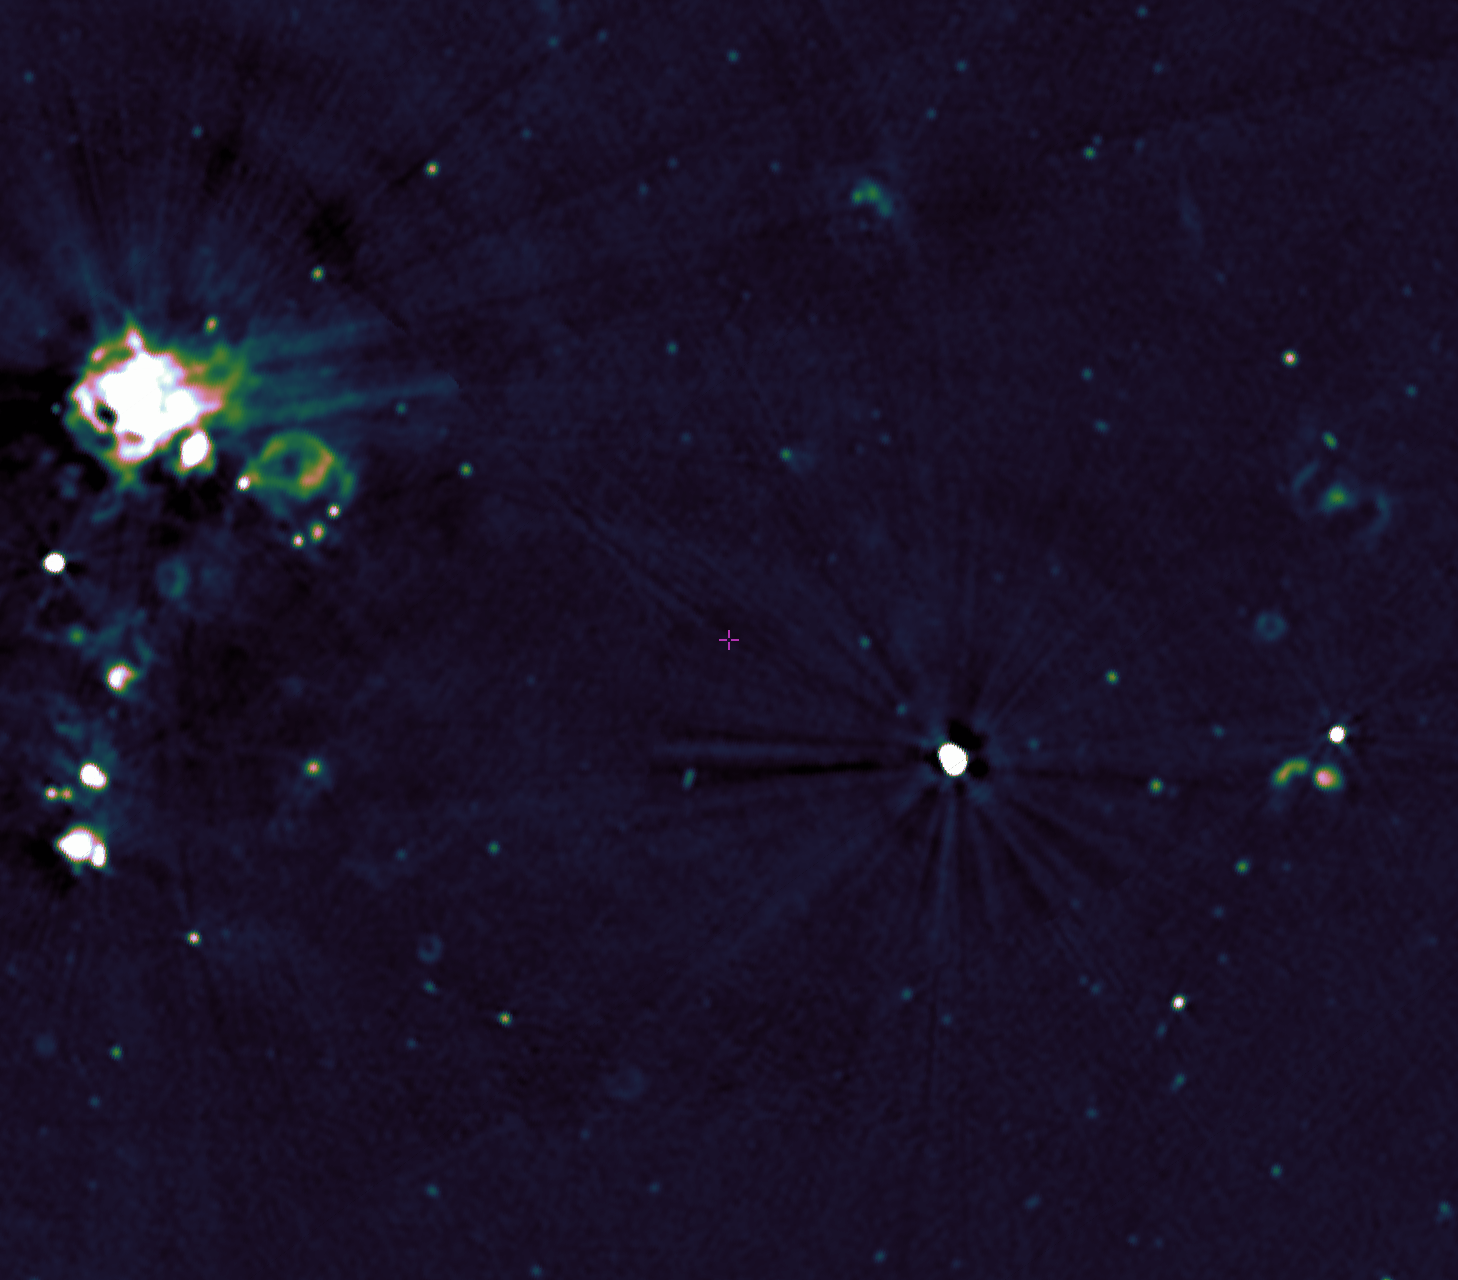
\includegraphics[width=1.0\linewidth]{./chapters/10.results/LMC/radio-843_cut.png}
		\caption{Radio wavelength at 843MHz.}
		\label{results:LMC:radio}
	\end{subfigure}
	\begin{subfigure}[b]{0.375\linewidth}
		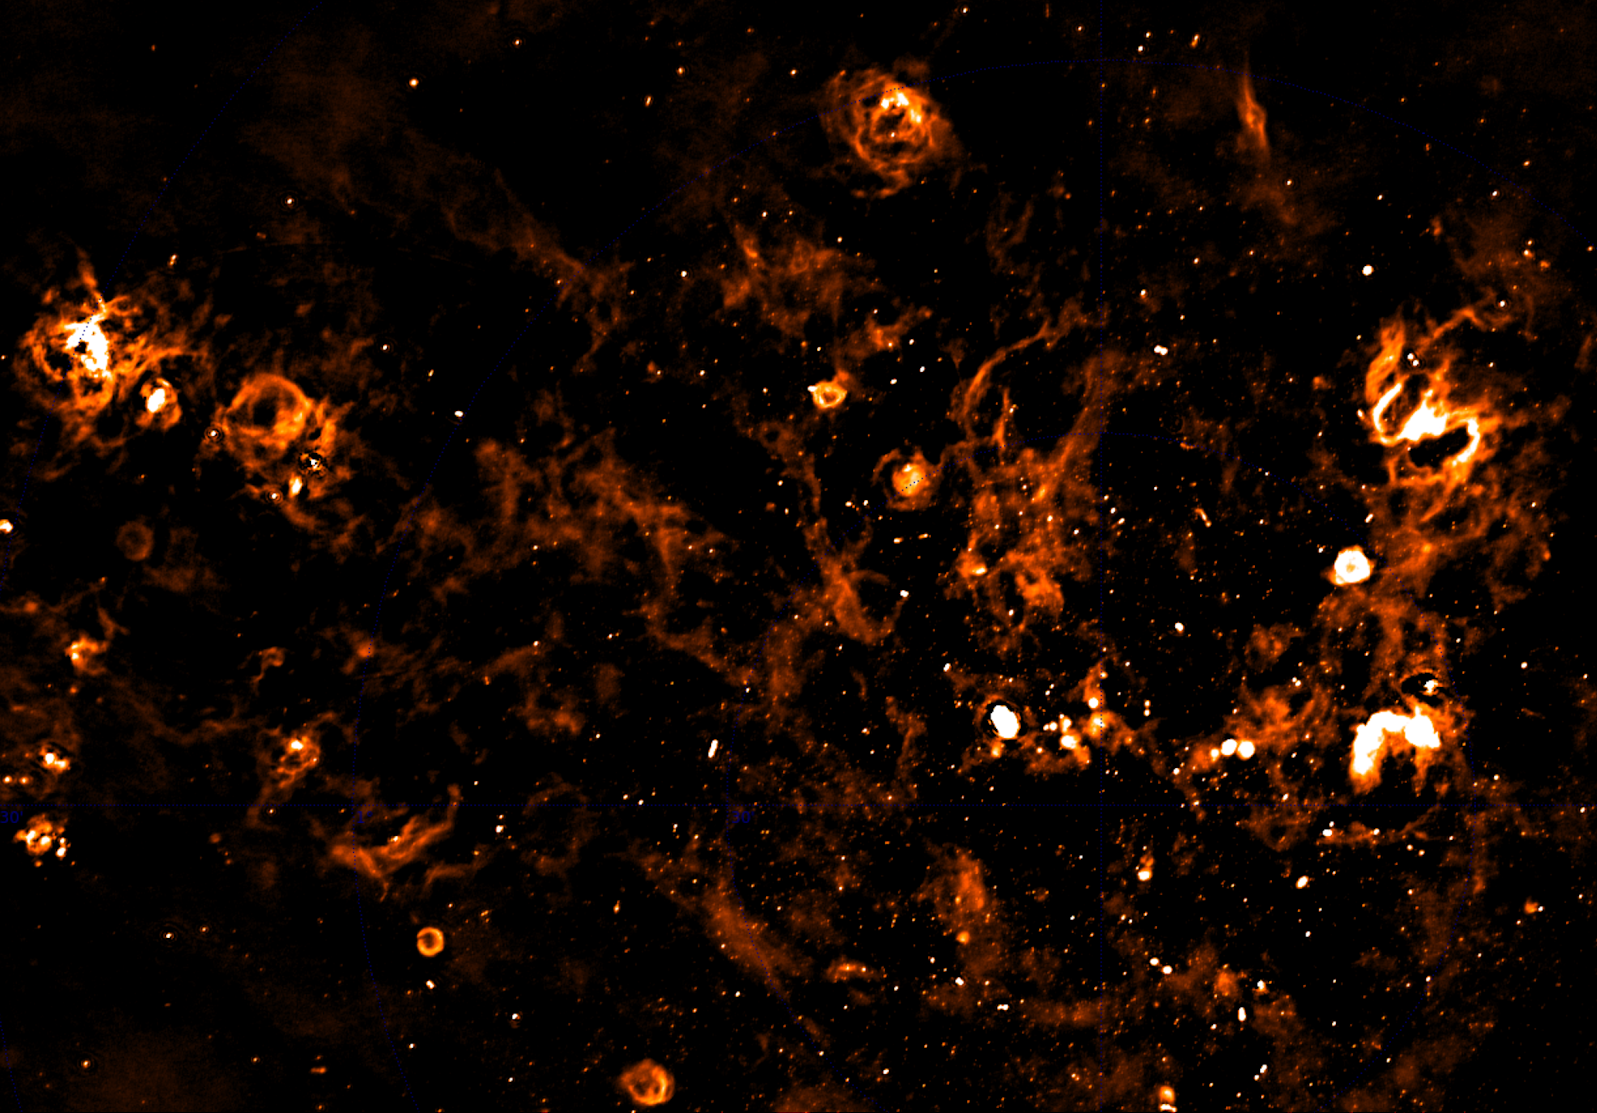
\includegraphics[width=1.0\linewidth]{./chapters/10.results/LMC/meerkat2.png}
		\caption{Wide band radio image by MeerKAT.}
		\label{results:LMC:meerkat}
	\end{subfigure}
	\caption{Section of the Large Magellanic Cloud (LMC)}
	\label{results:LMC}
\end{figure}

The MeerKAT observation covers a wide band of radio frequencies. The lowest frequency in the MeerKAT observation is 894 MHz, and the highest frequency is 1658 Mhz.
Imaging the whole frequency band requires a wide band deconvolution algorithm. In wide band imaging, several images at different frequencies get deconvolved as an image cube. Wide band imaging again multiplies the amount of work that has to be done for reconstruction, as now we cannot deconvolve a single image, but have to deal with a whole image cube.

Wide band imaging is not possible within the time frame of this project. We take a narrow band subset of 5 channels from the original data (ranging from 1084 to 1088 MHz, about 1 Gb in size) for reconstruction. We also reduce the field-of-view to a more manageable section. Figure \ref{results:cutout} shows the LMC image section we are using together with a CLEAN reconstruction of the narrow band data.

\begin{figure}[h]
	\centering
	\begin{subfigure}[b]{0.4\linewidth}
		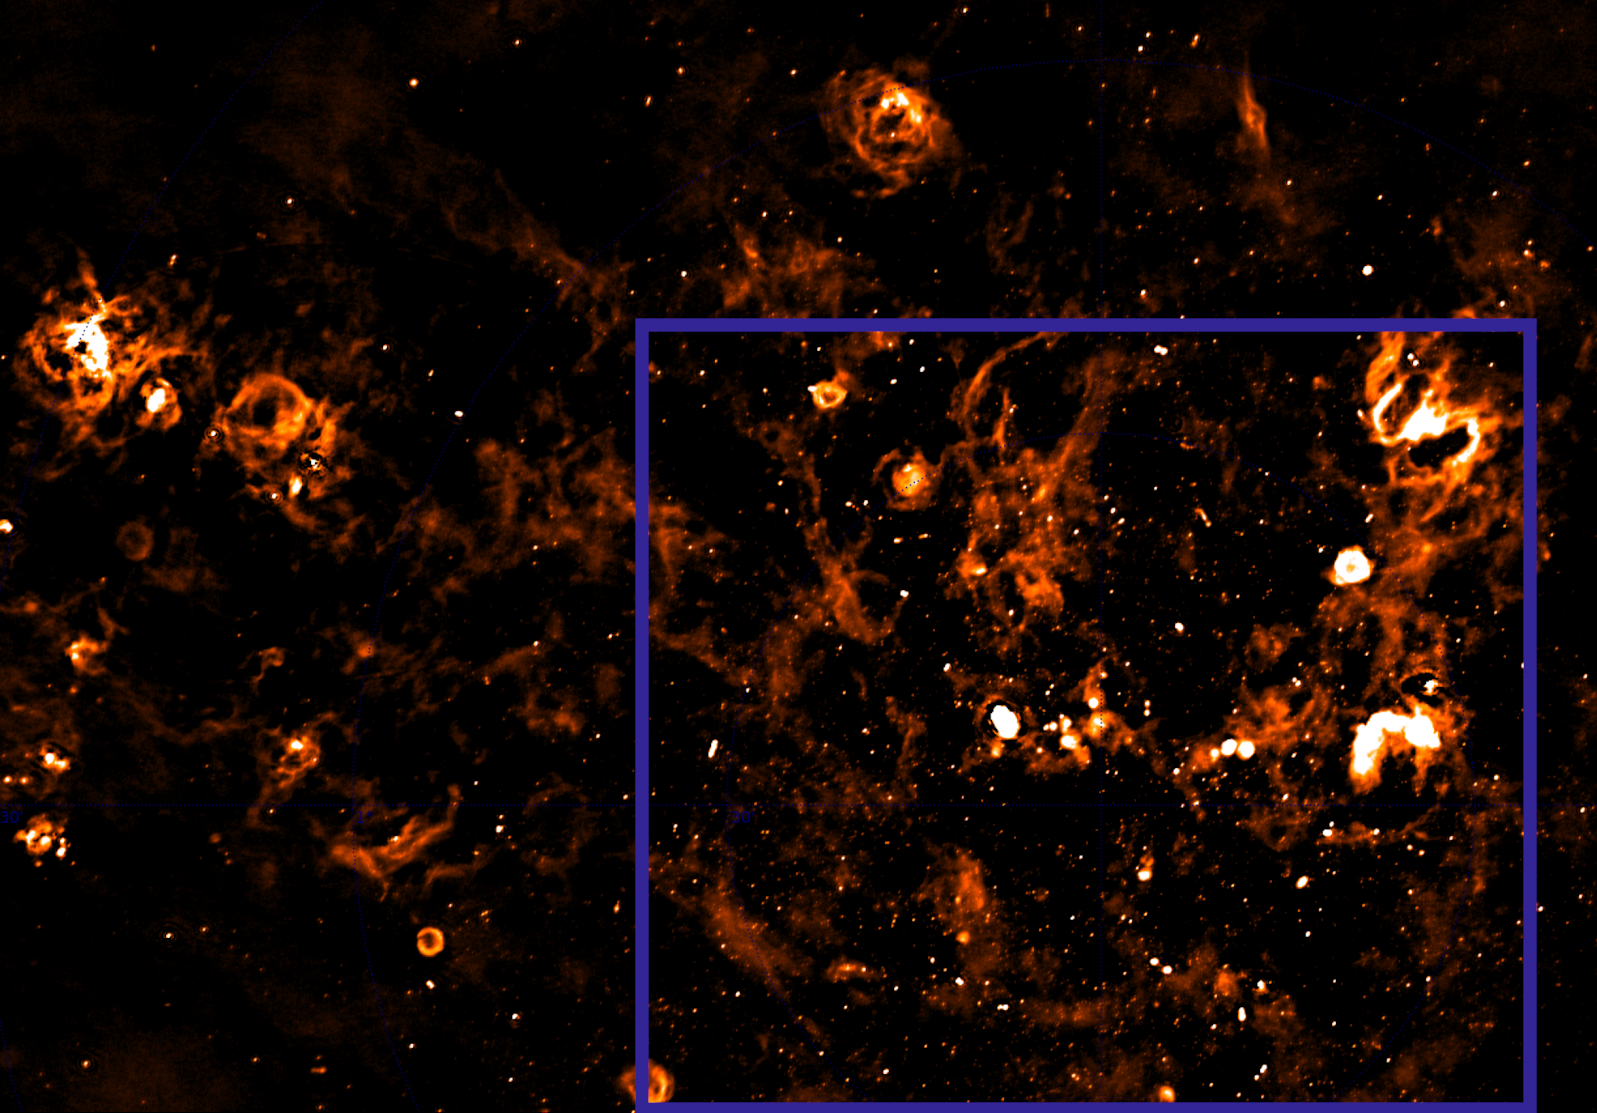
\includegraphics[width=1.0\linewidth]{./chapters/10.results/LMC/meerkat_cutout.png}
	\end{subfigure}
	\begin{subfigure}[b]{0.28\linewidth}
		\adjincludegraphics[width=1.0\linewidth, clip, trim={0.72in 0.72in 0.72in 0.72in}]{./chapters/10.results/MSClean/Natural-CLEAN.png}
	\end{subfigure}
	\caption{Narrow band image section used.}
	\label{results:cutout}
\end{figure}

At the center of our image section \ref{results:cutout} we see the N132D supernova remnant. We partially see the faint extended emissions, although they are close to the noise level. This is known as a high-dynamic range reconstruction. We have strong radio sources mixed together with faint emissions, which are only marginally above the noise level of the image.

The total field-of-view of our image section is roughly 1.3 degrees(or 4600 arc seconds). Our reconstruction has $3072^2$ pixel with a resolution of 1.5 arc seconds per pixel. this is still a wide field-of-view reconstruction problem. We have to account for the effects of the $w$-term to achieve a high-dynamic range reconstruction.

In our test reconstruction, we need to account for $w$-term correction and high-dynamic range. We have excluded wide-band imaging as not feasible within the time frame of this project. In Section \ref{results:cleancomp} we compare the reconstructions of CLEAN with our serial coordinate descent algorithm on the LMC observation. The next Section \ref{results:speedup} presents the speedup we achieve with serial coordinate descent by using our distributed or GPU-accelerated implementations.

In Section \ref{results:gradients} we show the core result of this project. Namely what effect has an approximate $PSF$ on the deconvolution problem and whether we can use it to further distribute the problem. The answer to that question is affirmative: We can approximate the $PSF$, and we can exploit it to further distribute the deconvolution. But we need more sophisticated coordinate descent algorithms to fully benefit from it.


\subsection{Comparison with CLEAN reconstructions} \label{results:cleancomp}
We use the WSCLEAN \cite{offringa2014wsclean} implementation of multi-scale CLEAN algorithm. We compare our coordinate descent reconstruction with two CLEAN reconstructions, oe with naturally weighted visibilities and one with briggs-weighted visibilities.

There are three main visibility weighting scheme for the gridder that lead to different $PSF$s from the same measurements: Natural, uniform, and Briggs\cite{briggsWeighting}. Natural weighting scheme leads to an image with a lower noise level, but a wider $PSF$. Uniform weighting leads to a higher noise level, but to a $PSF$ which is more concentrated around a single pixel. Briggs weighting is a scheme combines the best from both worlds, receiving an image with acceptable noise level while getting a more concentrated $PSF$. As such it is widely used in radio astronomy image reconstruction. Our gridder implements the natural weighting scheme only. Nevertheless our coordinate descent algorithm is able to retrieve structures similar to the briggs-weighted multi-scale CLEAN reconstruction, even though coordinate descent has to work with a wider $PSF$.

Figure \ref{results:cleancomp:figure} shows the reconstruction of both briggs-weighted multi-scale CLEAN and the naturally weighted coordinate descent reconstruction. We used a regularization parameter of $\lambda = 1.0 * Lipschitz$ and $\alpha = 0.01$. The elastic net regularization is biased heavily towards the L2 norm. We stopped the serial coordinate descent if every possible pixel change is below $\epsilon = 1e^{-5}$. We use these parameters for the whole project unless we specify otherwise.

\newpage

\begin{figure}[!htp]
	\centering
	\begin{subfigure}[b]{0.950\linewidth}
		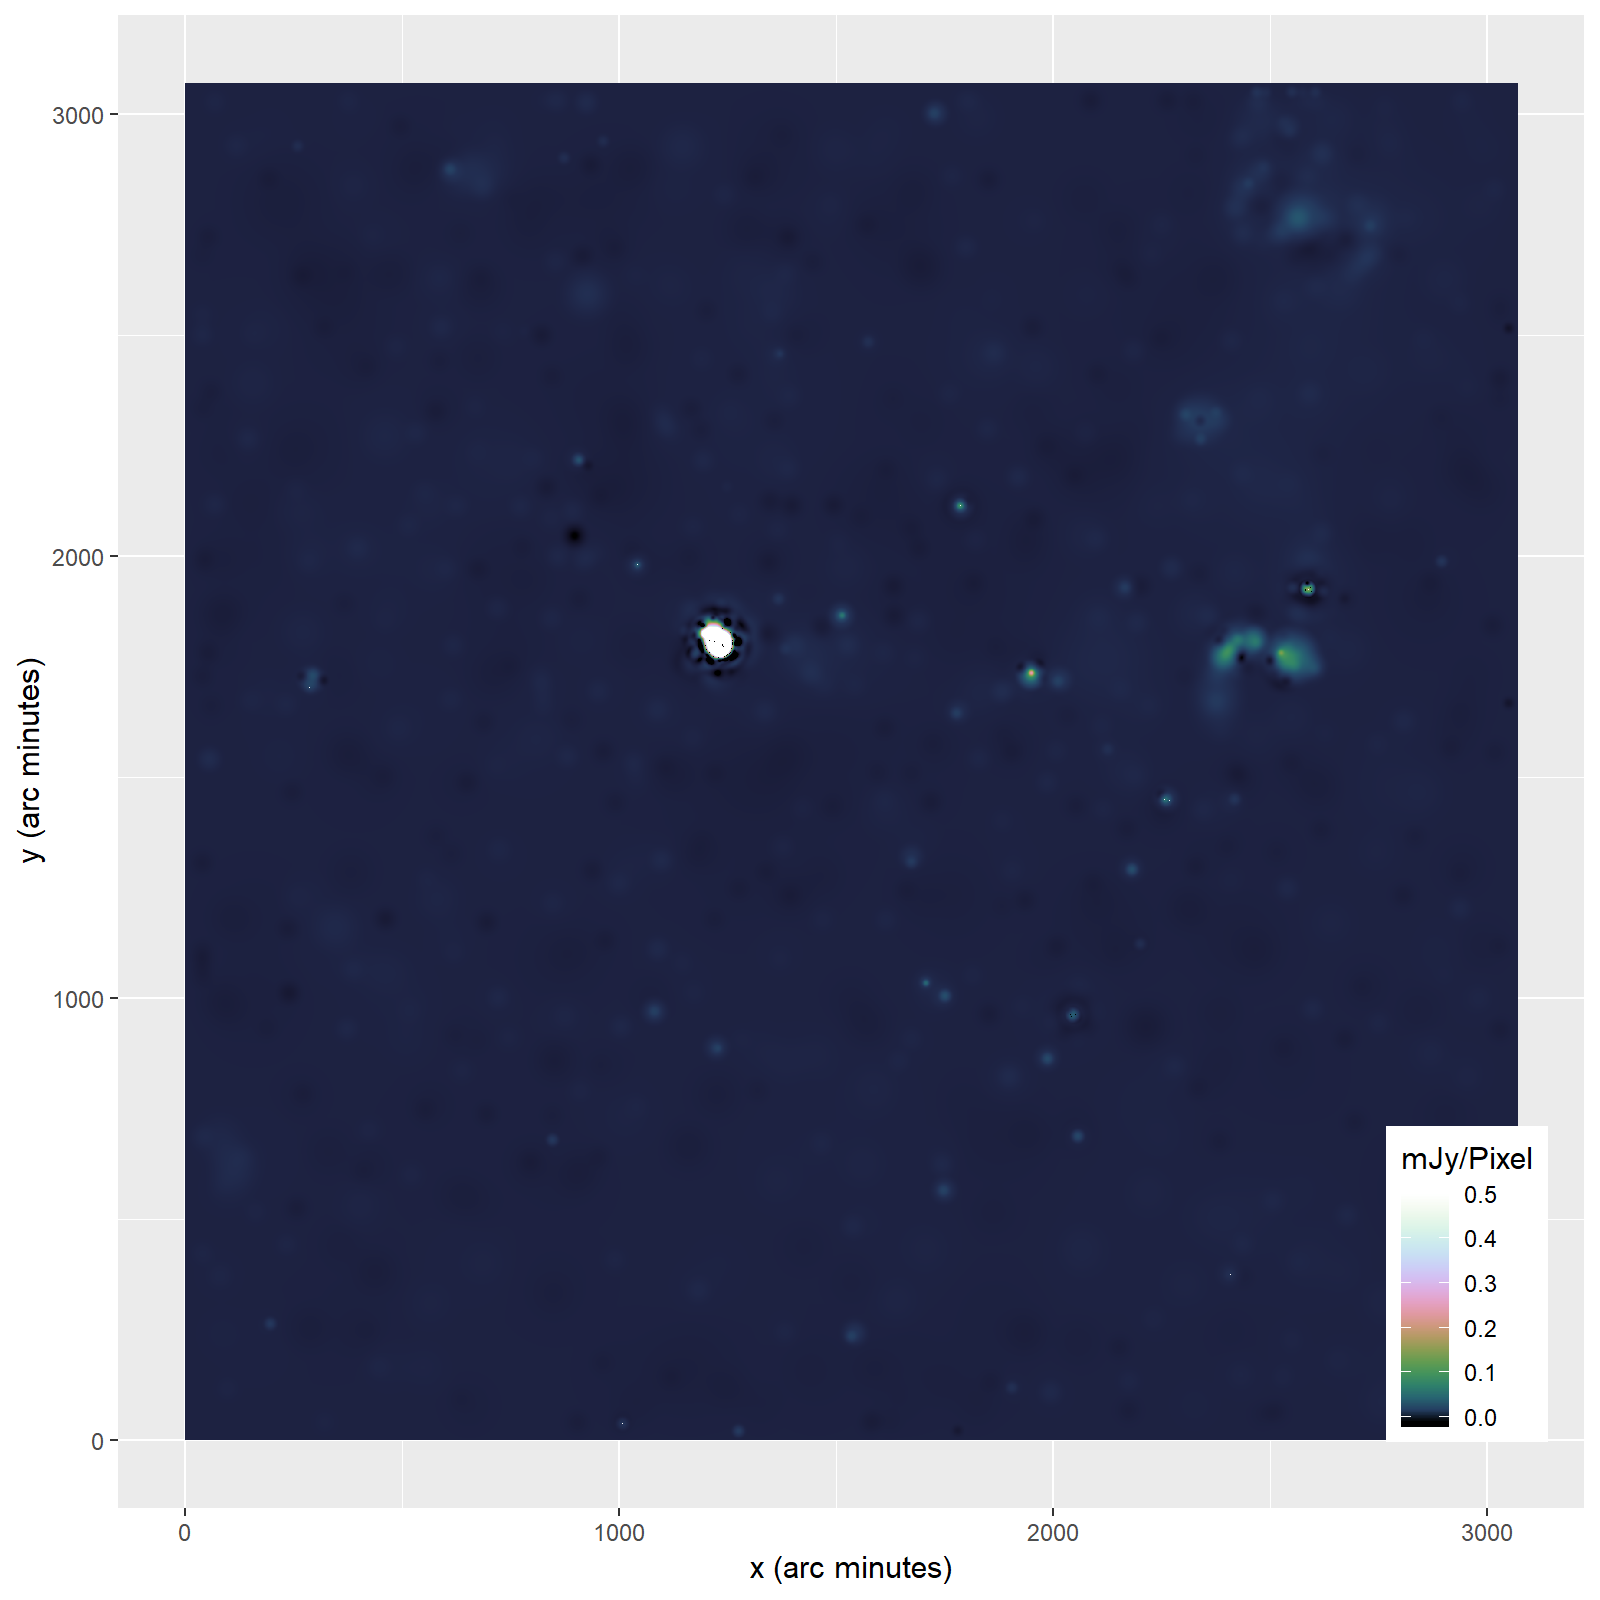
\includegraphics[width=0.412\linewidth, clip, trim={0.72in 0.72in 0.72in 0.72in}]{./chapters/10.results/MSClean/Natural-CLEAN.png}
		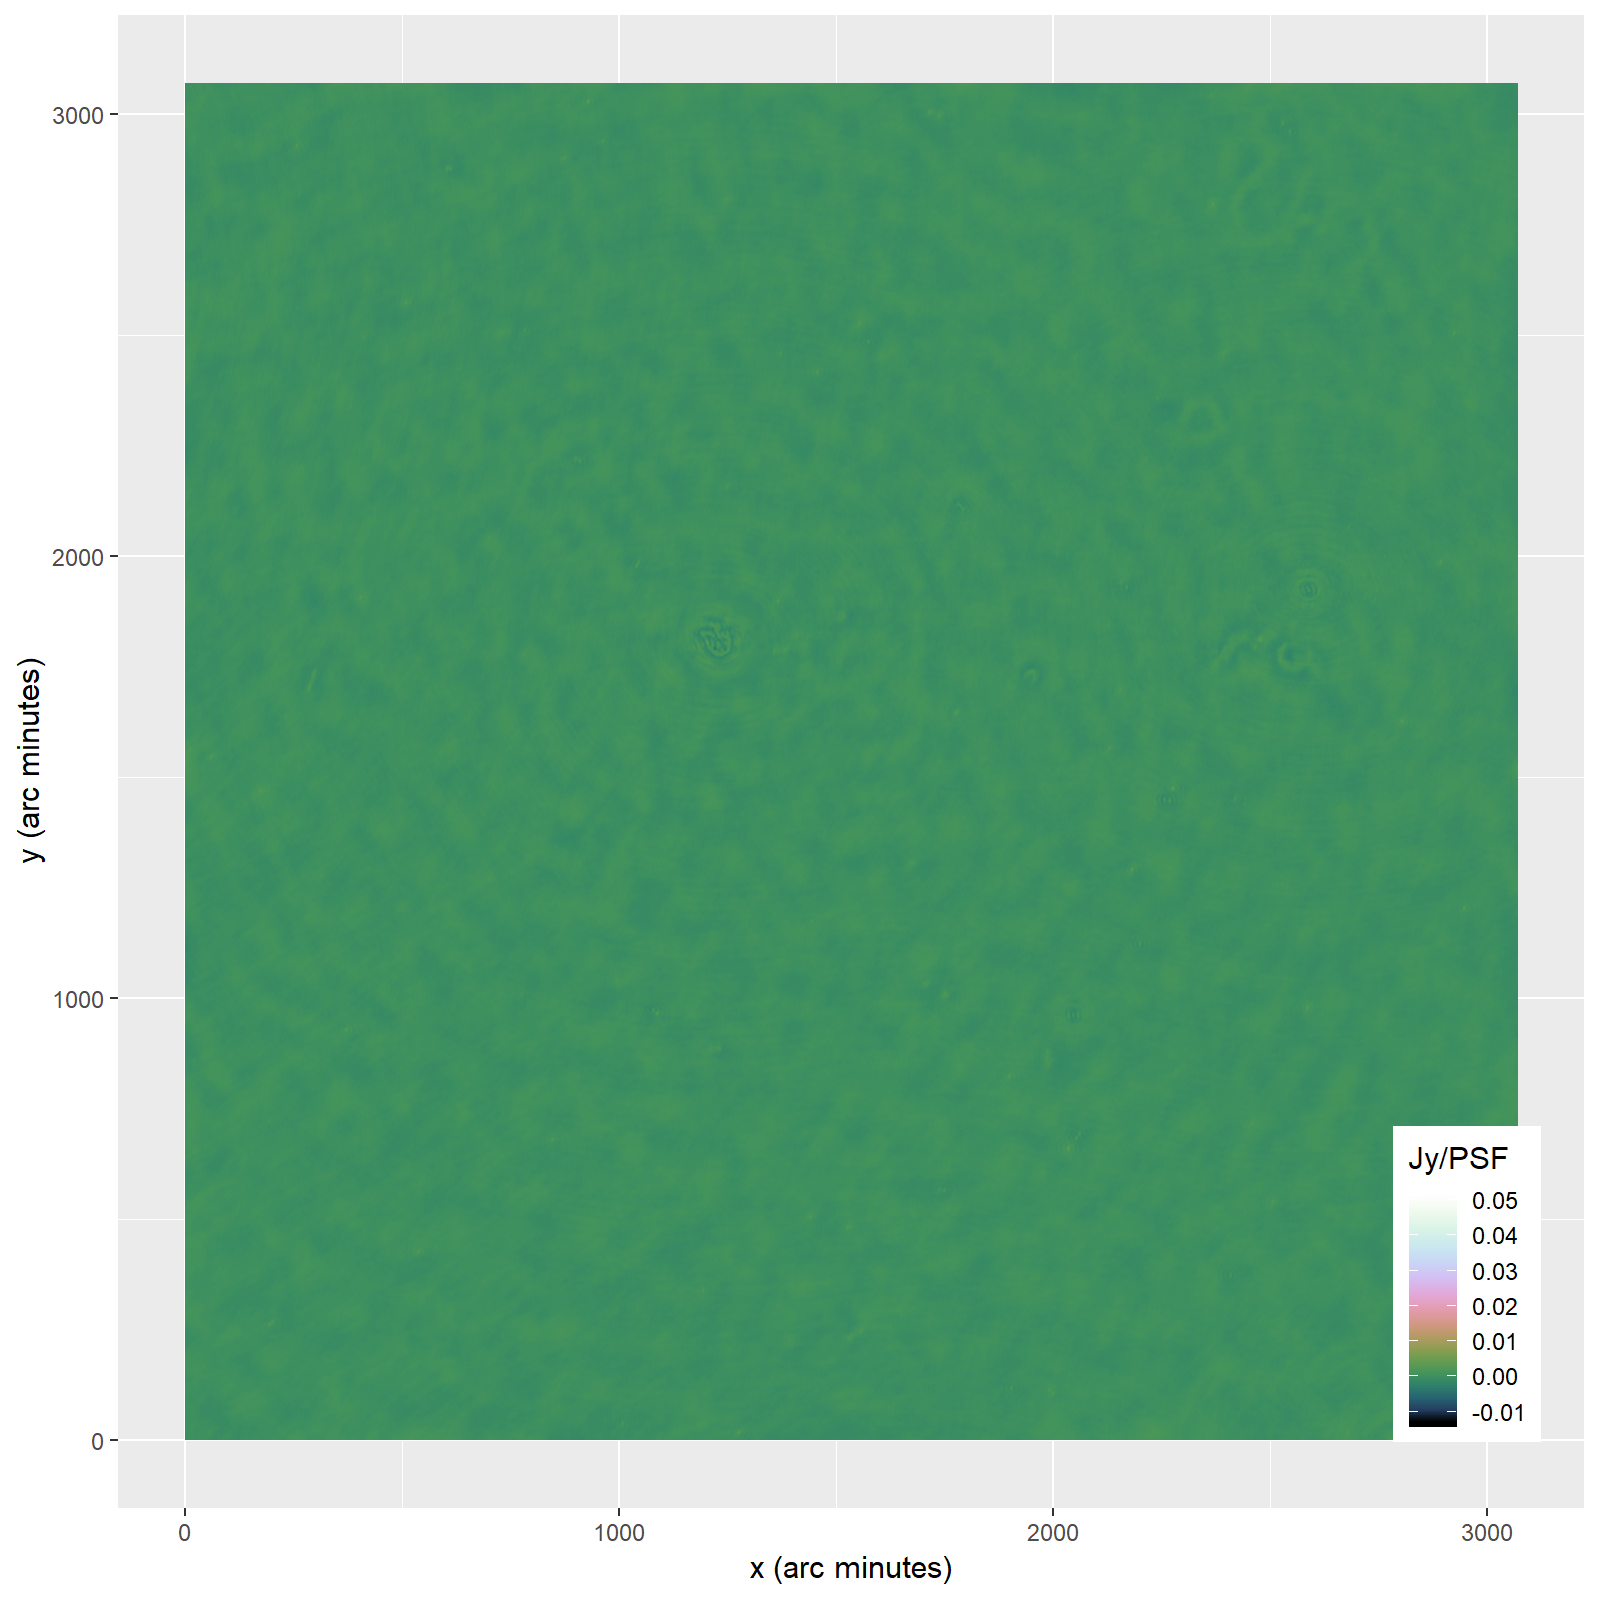
\includegraphics[width=0.490\linewidth, clip, trim={0.36in 0.36in 0.0in 0.36in}]{./chapters/10.results/MSClean/Natural-CLEAN-residuals.png}
		\caption{Multi-scale CLEAN.}
		\label{results:comp:clean}
	\end{subfigure}
	\begin{subfigure}[b]{0.95\linewidth}
		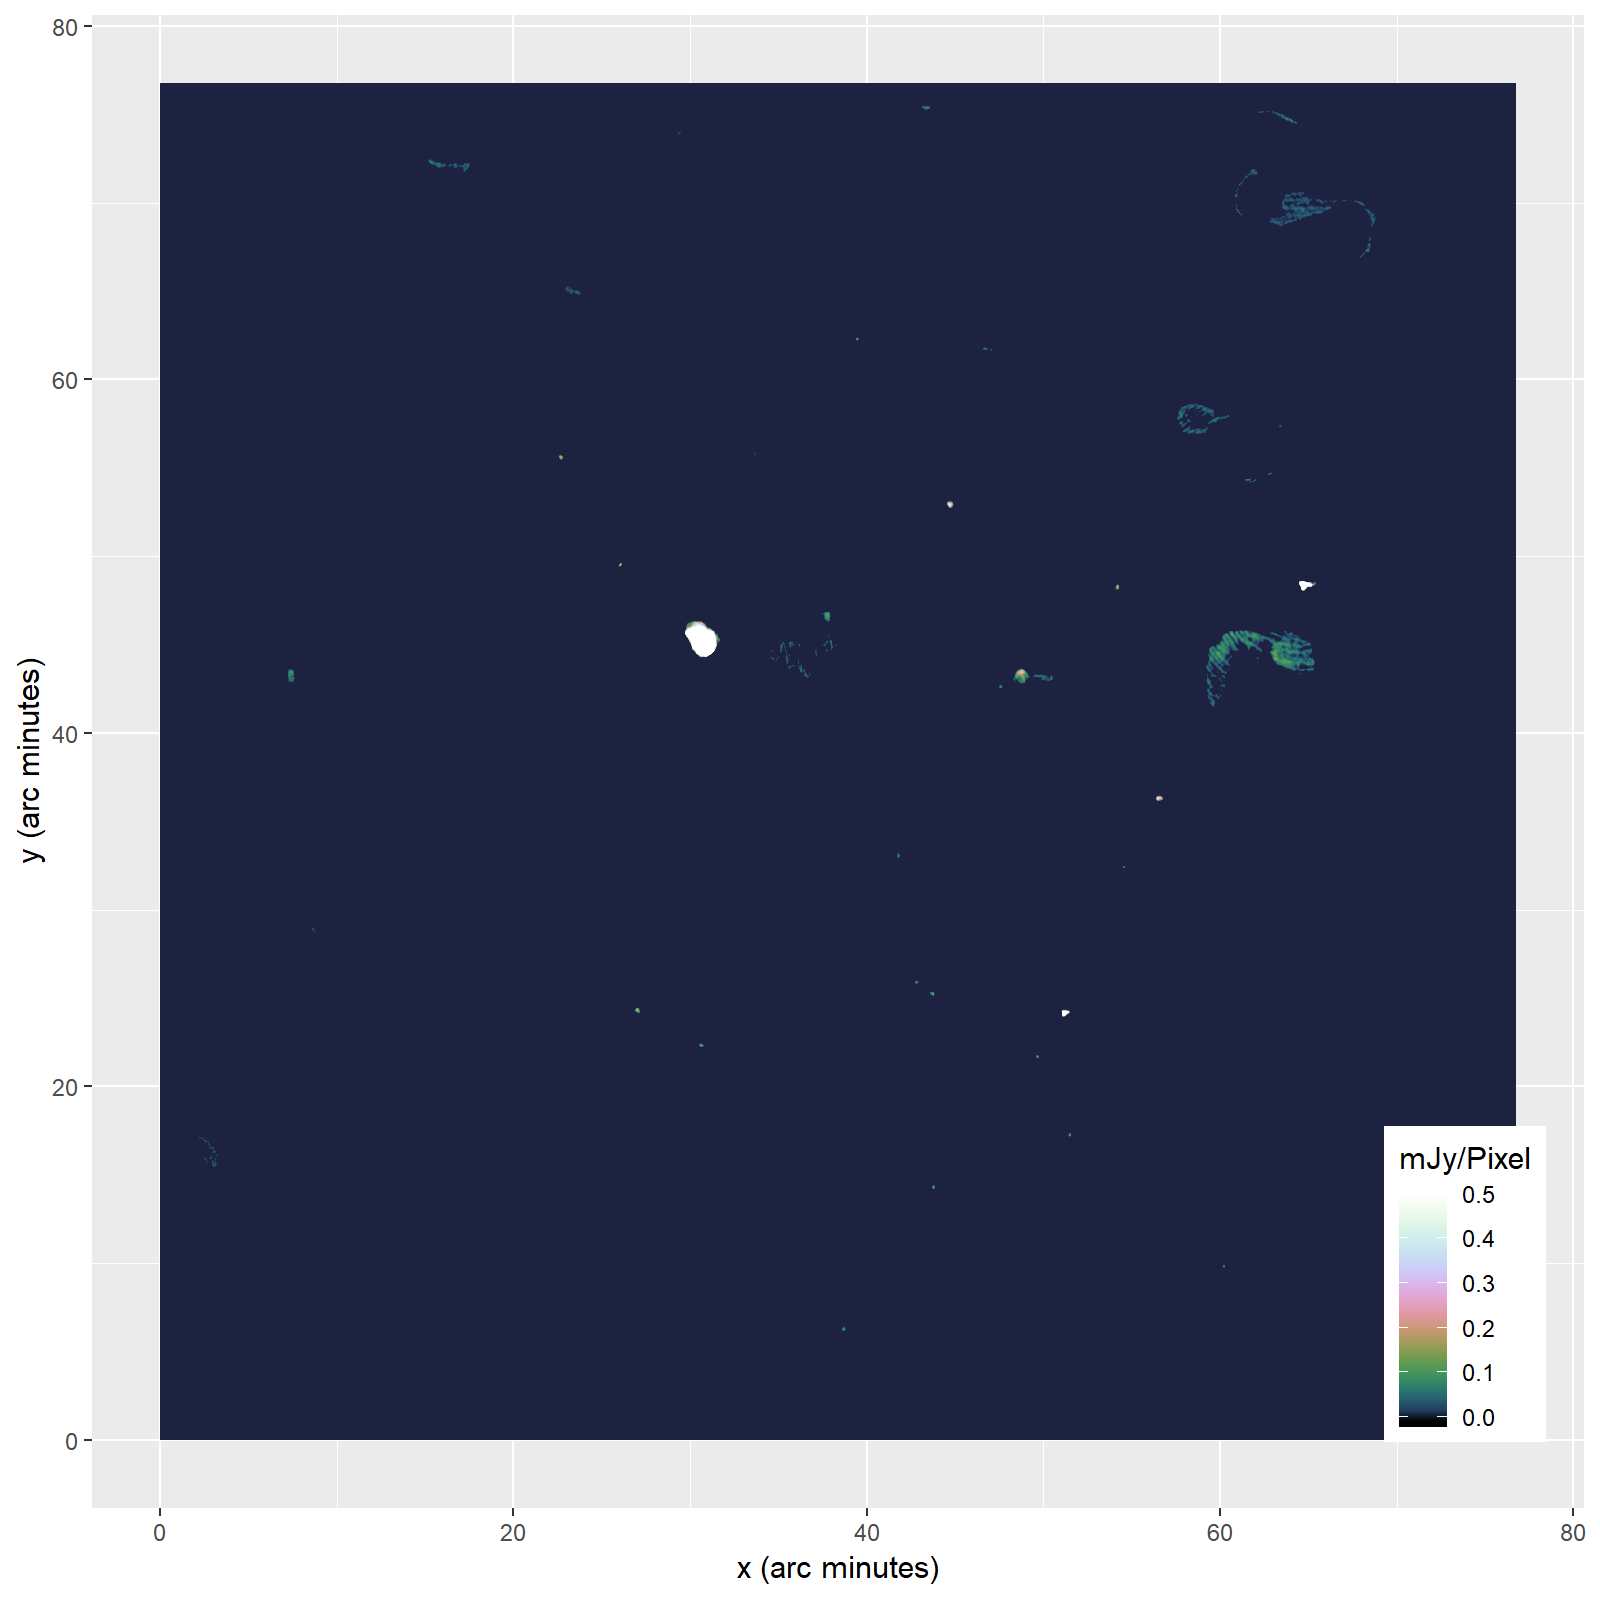
\includegraphics[width=0.412\linewidth, clip, trim={0.72in 0.72in 0.72in 0.72in}]{./chapters/10.results/SerialCD/CD-reference.png}
		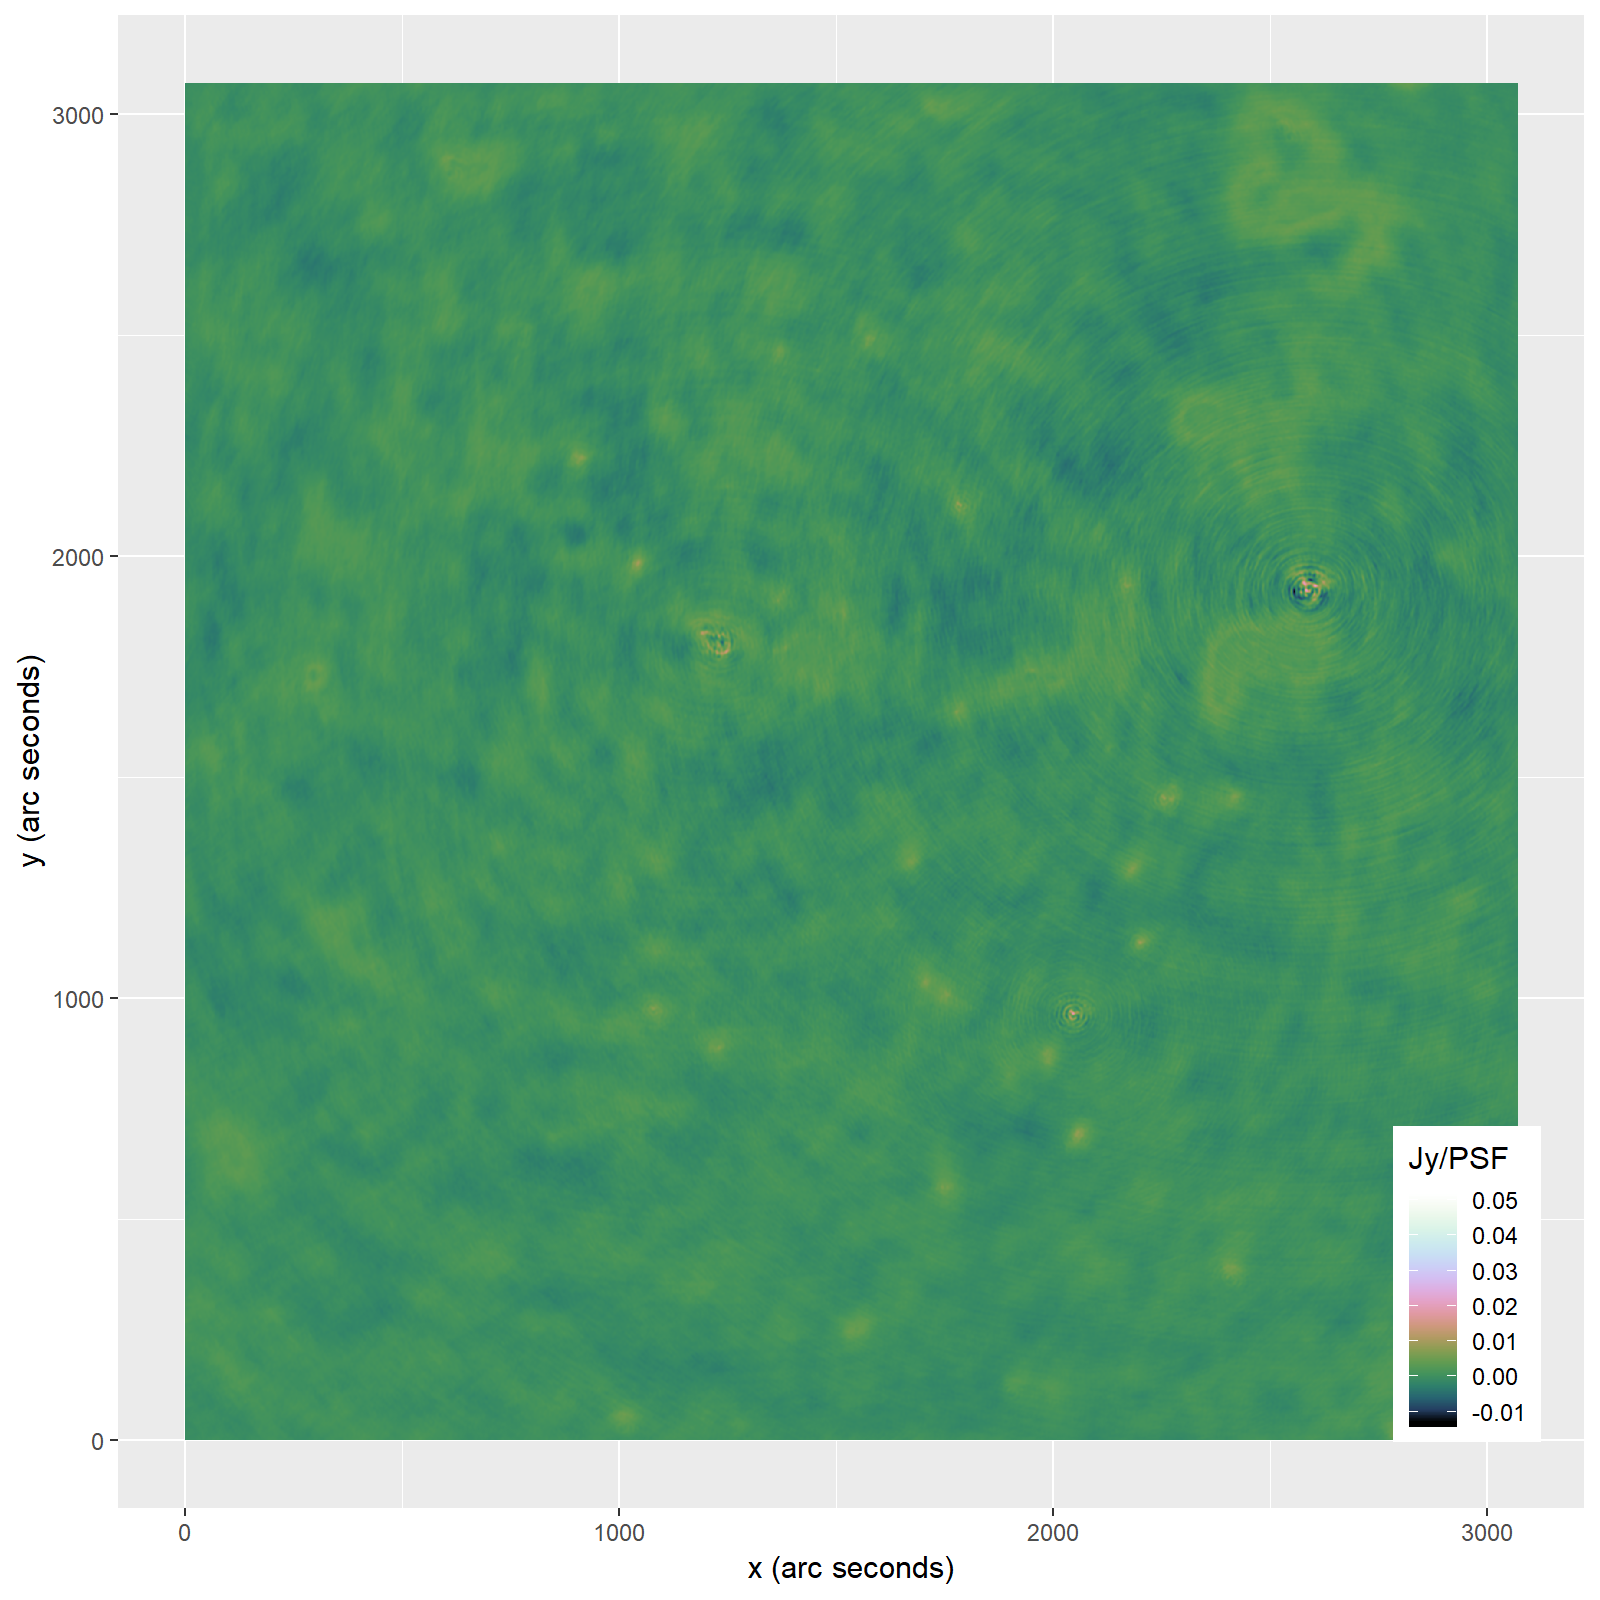
\includegraphics[width=0.490\linewidth, clip, trim={0.36in 0.36in 0.0in 0.36in}]{./chapters/10.results/SerialCD/CD-reference-residuals.png}
		\caption{Serial coordinate descent.}
		\label{results:comp:clean}
	\end{subfigure}
	\begin{subfigure}[b]{0.95\linewidth}
		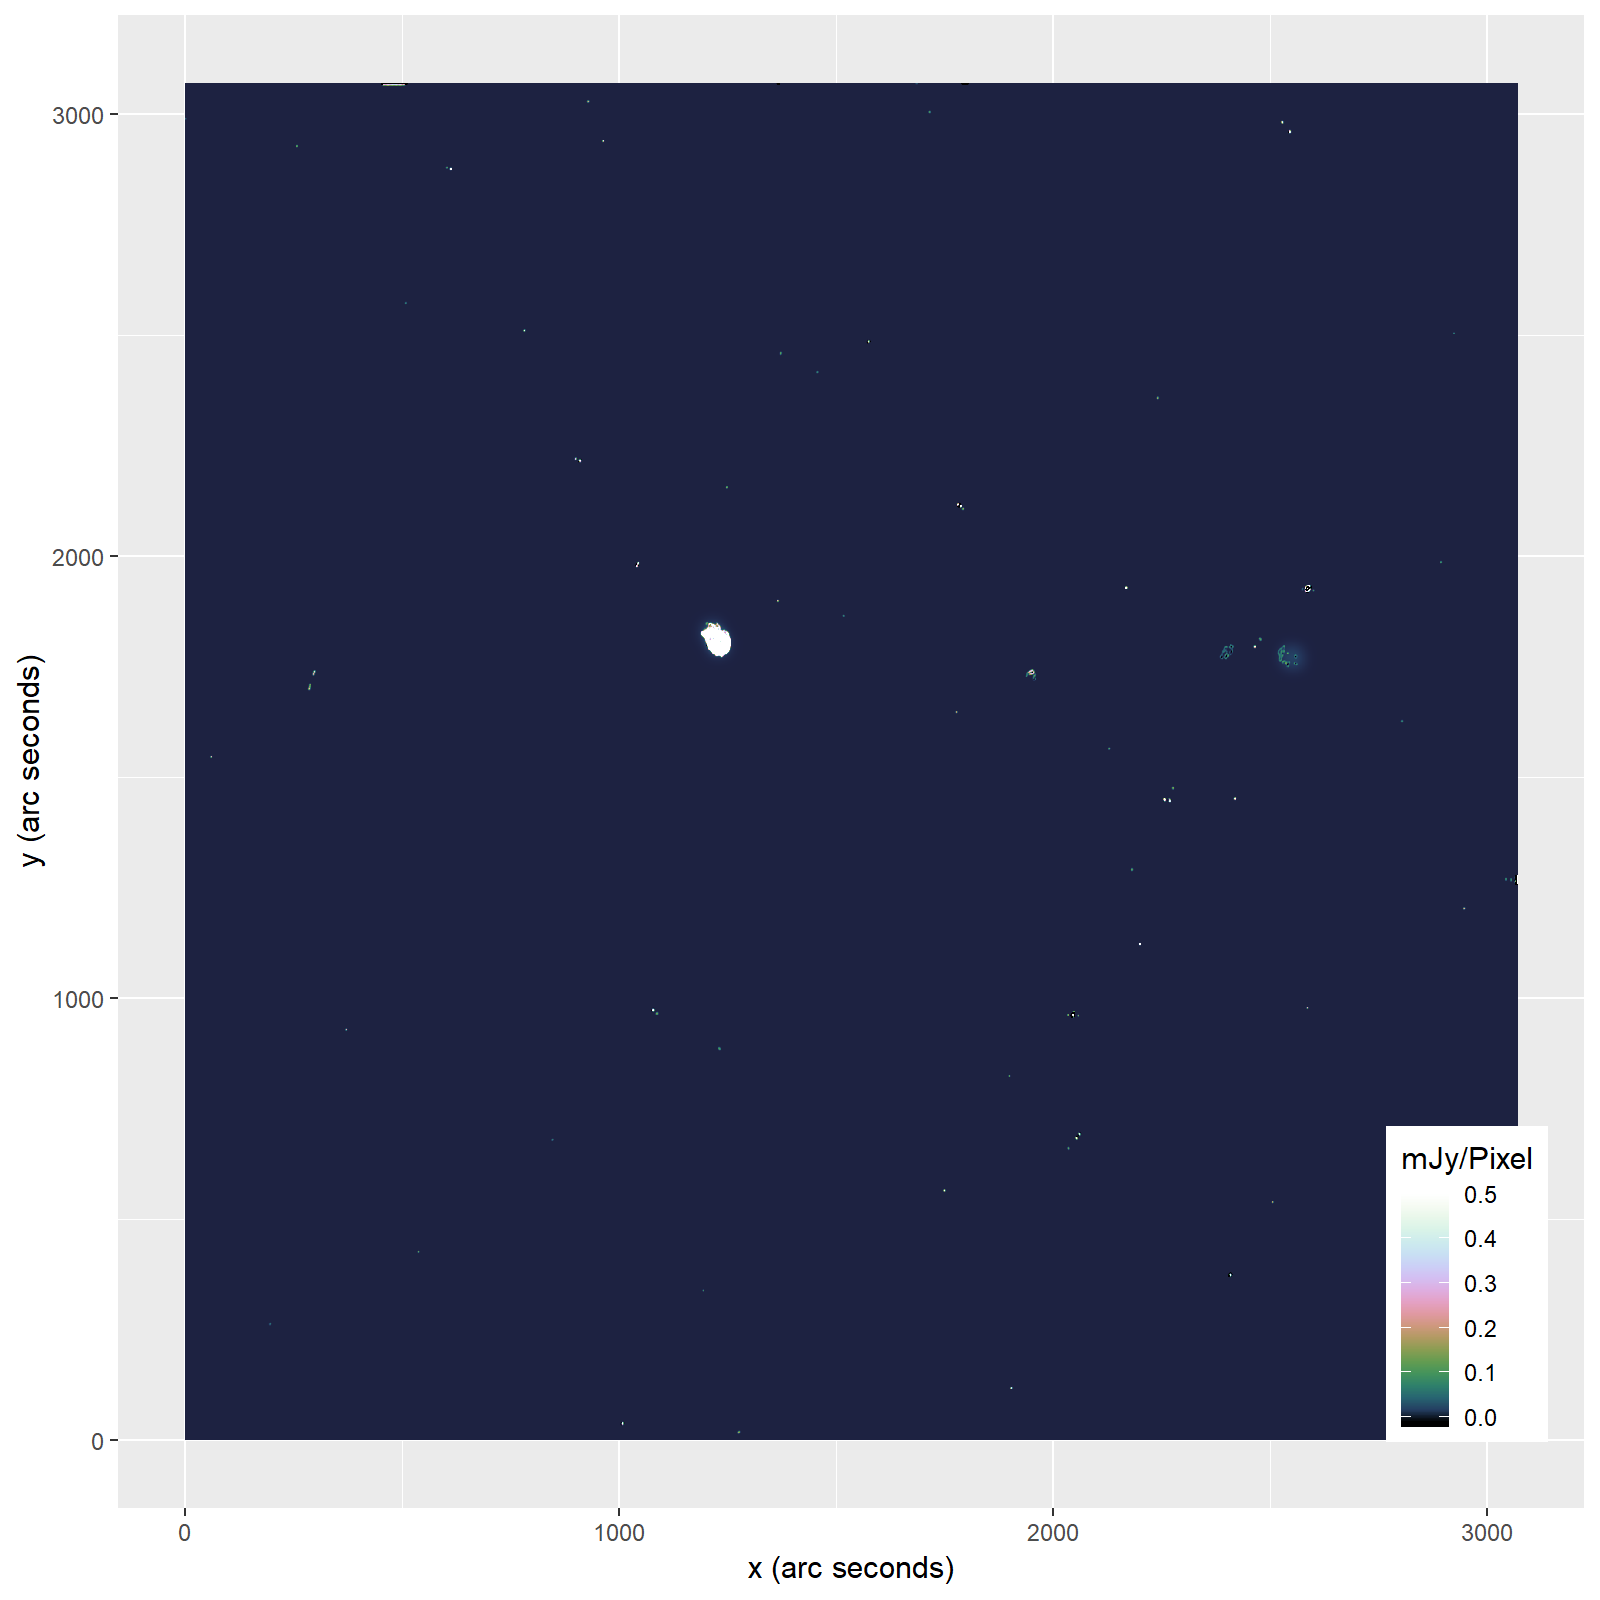
\includegraphics[width=0.412\linewidth, clip, trim={0.72in 0.72in 0.72in 0.72in}]{./chapters/10.results/iuwt/iuwt-model.png}
		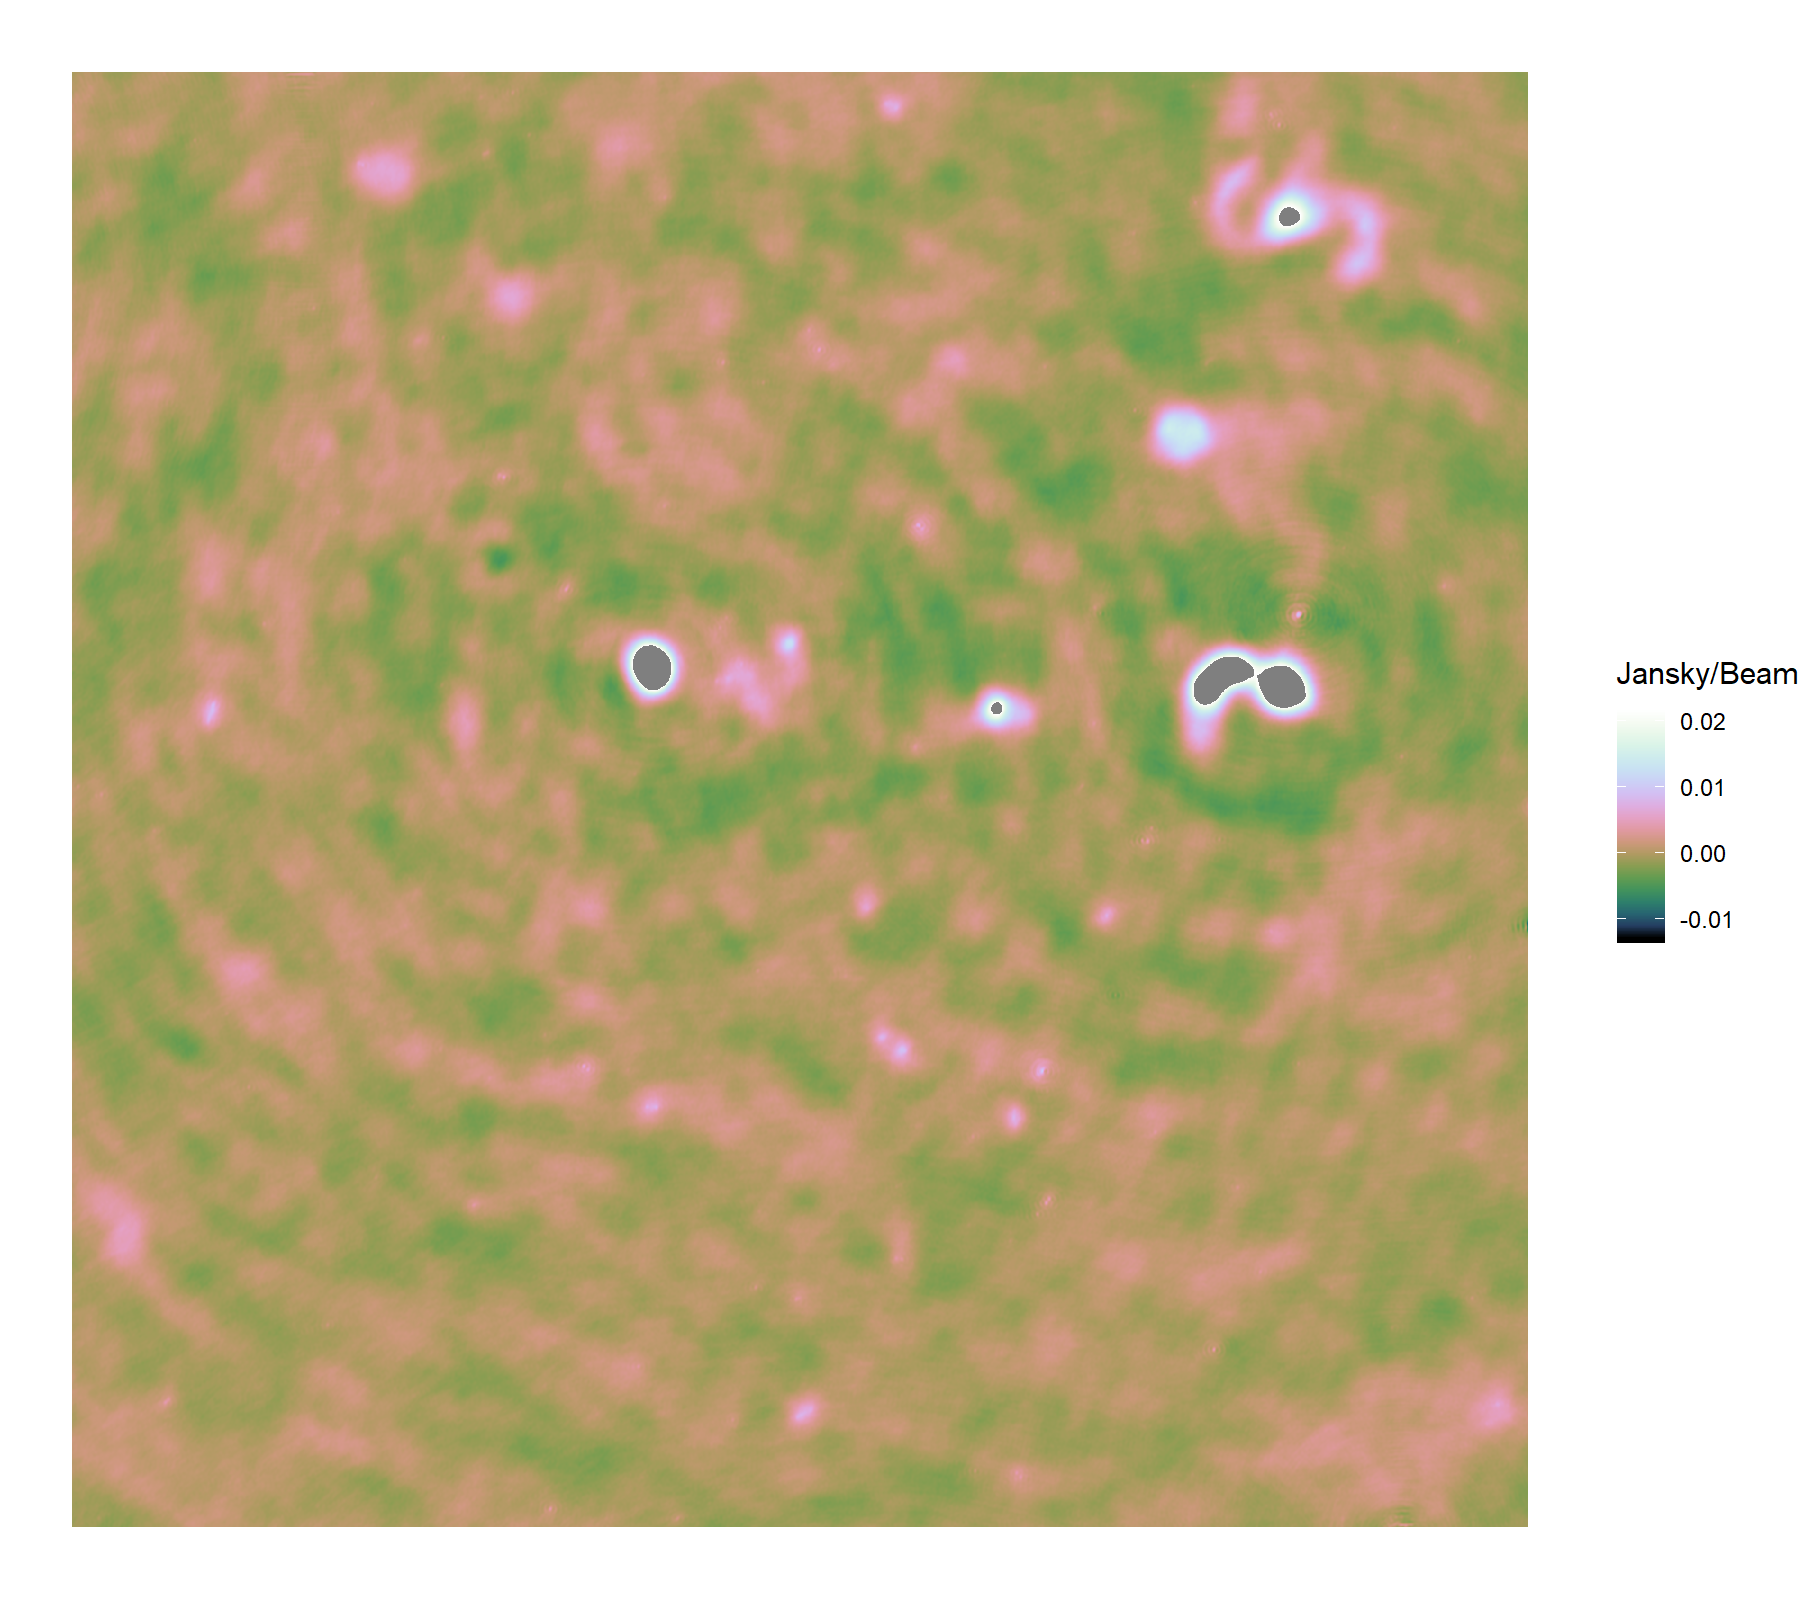
\includegraphics[width=0.490\linewidth, clip, trim={0.36in 0.36in 0.0in 0.36in}]{./chapters/10.results/iuwt/iuwt-residuals.png}
		\caption{MORESANE (IUWT).}
		\label{results:comp:clean}
	\end{subfigure}

	\caption{Comparison of the whole image}
	\label{results:cleancomp:figure}
\end{figure}

\newpage

Multi-scale reconstructed its image within 6 Major and 14 thousand Minor cycle iterations. Our serial coordinate descent algorithm converged after 5 Major cycles and used 100 thousand iterations to converge. Our algorithm required roughly 8 times more iterations. It took a total of 35 minutes to reconstruct an image on an Intel Xeon E3-1505M with 8 logical cores. On this data set, our algorithm used one Major cycle less than multi-scale CLEAN. However, the number of Major cycles is not directly comparable. We do not use the identical criteria to initiate another Major cycle: At the beginning of each deconvolution, we check the maximum pixel difference. If it is below $\epsilon_{major} = 1e^{-4}$, we stop the reconstruction. We have not compared our stopping criterion to WSCLEAN. As such, the number of Major cycles are only a rough comparison. Our serial coordinate descent uses a similar number of Major cycles as multi-scale CLEAN.

Both algorithms detect the three extended emissions at the right side of the image. They detect various point sources at the same location. Coordinate descent and multi-scale CLEAN arrive at a roughly similar result. Coordinate descent detects similar structures in the N132D supernova remnant, as the briggs-weighted CLEAN, but also includes calibration errors in its reconstruction of the faint extended emissions.

When we compare the reconstruction quality of multi-scale CLEAN an our serial coordinate descent algorithm, we note that the magnitudes of the residual image of multi-scale CLEAN \ref{results:comp:clean-res} is significantly lower than the magnitudes in our algorithm, shown in \ref{results:comp:cd-res}. In the residual image of the serial coordinate descent algorithm, we still see some emissions belonging to stars, or extended emissions. This is to be expected, as multi-scale CLEAN uses several heuristics developed specifically for radio interferometric imaging\cite{offringa2017optimized}. 
%Describe Masking
Note however that the serial coordinate descent algorithm leaves large negative values in the residual image, while multi-scale CLEAN includes it in its reconstruction. Multi-scale CLEAN has several areas of negative pixel values, which is implausible.


\begin{figure}[h]
	\centering
	\begin{subfigure}[b]{0.32\linewidth}
		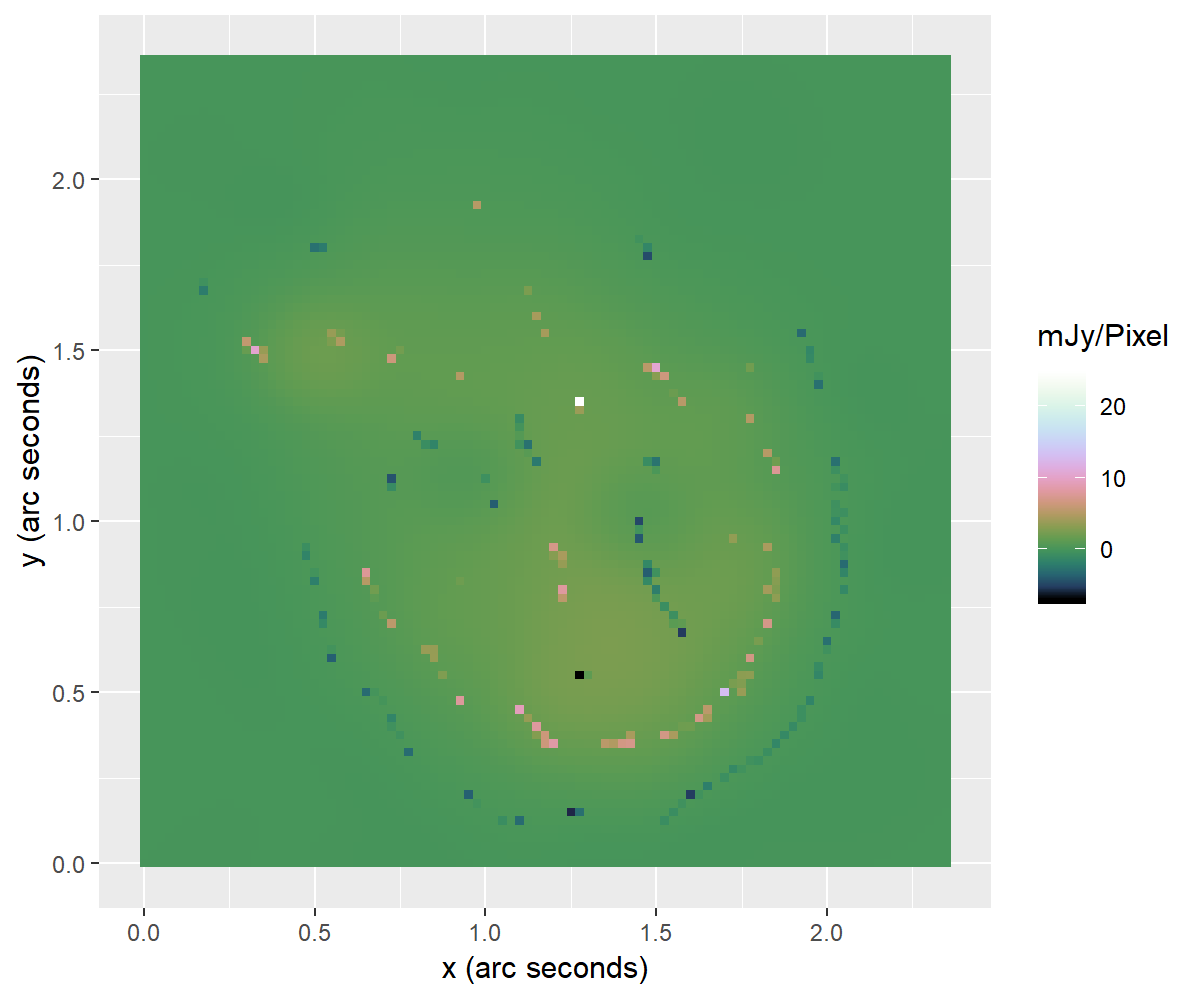
\includegraphics[width=1.00\linewidth]{./chapters/10.results/MSClean/Natural-N132.png}
		\caption{CLEAN Natural weighting.}
		\label{results:N132:clean}
	\end{subfigure}
	\begin{subfigure}[b]{0.32\linewidth}
		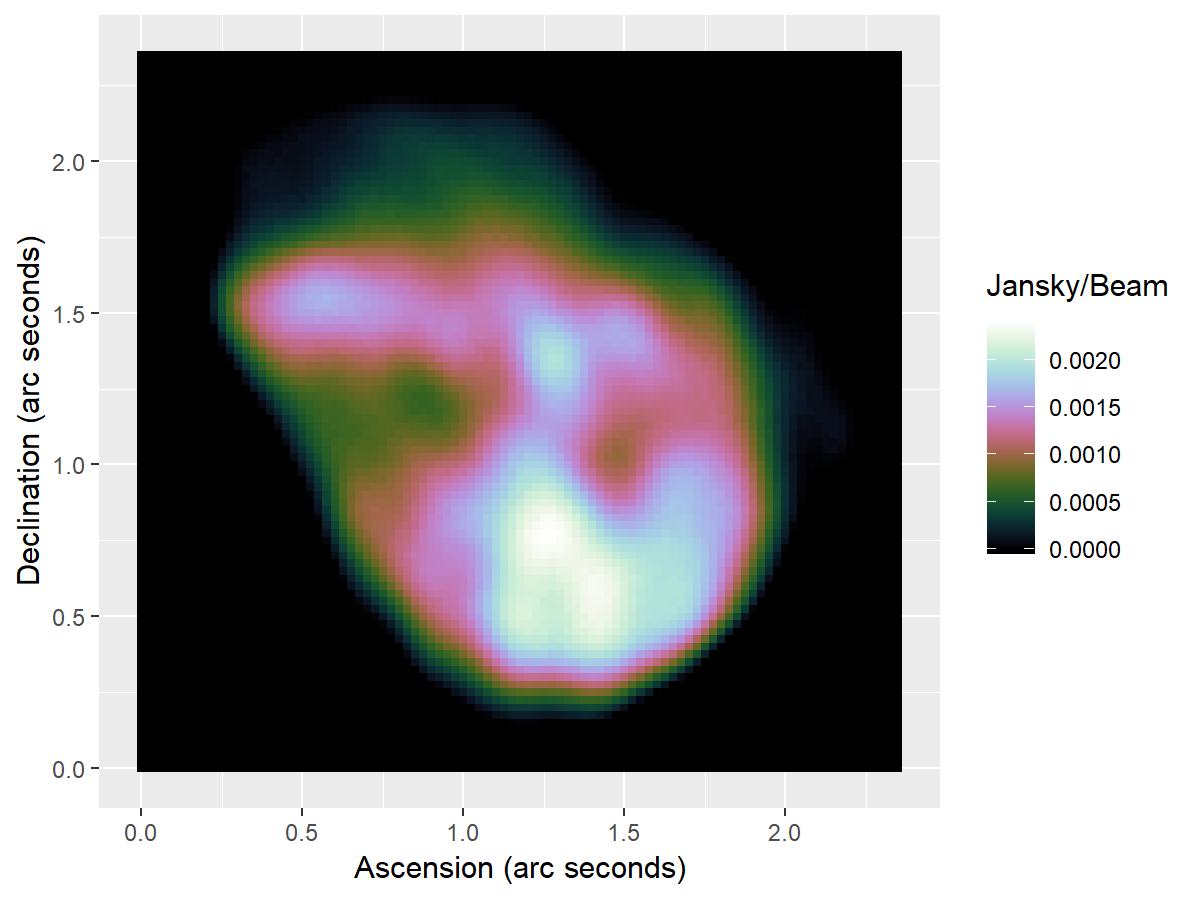
\includegraphics[width=1.00\linewidth]{./chapters/10.results/SerialCD/CD-N132.png}
		\caption{CD Natural weighting.}
		\label{results:comp:N132:cd}
	\end{subfigure}
	\begin{subfigure}[b]{0.32\linewidth}
		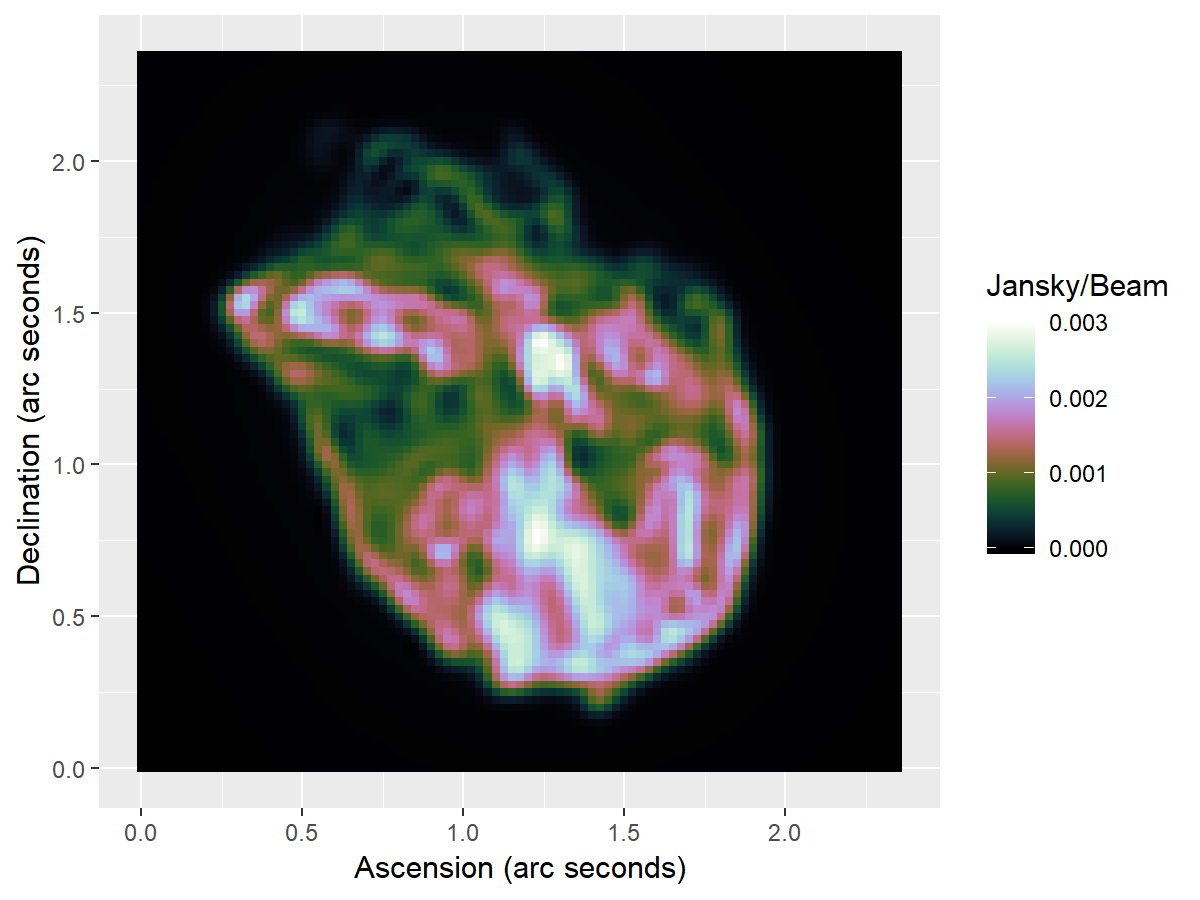
\includegraphics[width=1.00\linewidth]{./chapters/10.results/iuwt/iuwt-N132}
		\caption{CD Natural weighting.}
		\label{results:comp:N132:cd}
	\end{subfigure}
	\begin{subfigure}[b]{0.32\linewidth}
		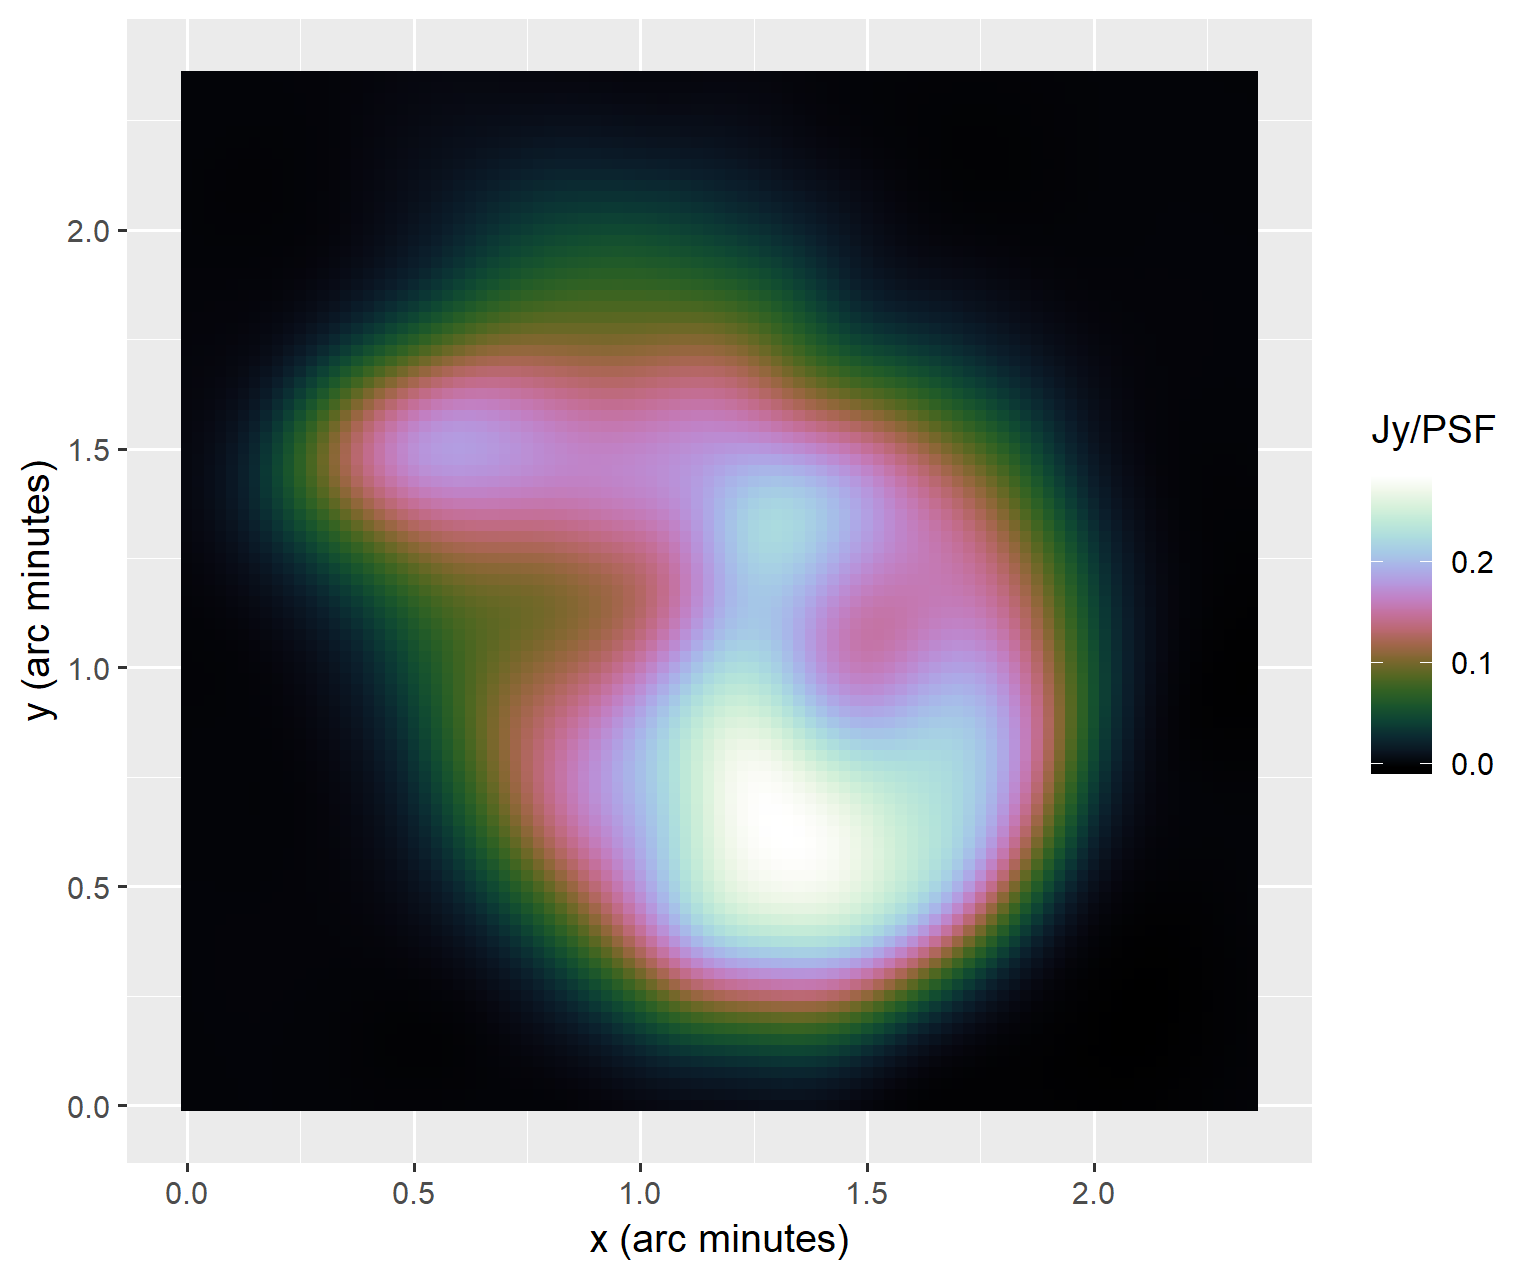
\includegraphics[width=1.00\linewidth]{./chapters/10.results/MSClean/Briggs-N132.png}
		\caption{CLEAN Briggs weighting.}
		\label{results:N132:cleanbriggs}
	\end{subfigure}
	\caption{N132D comparison}
	\label{results:cleancomp::N132:figure}
\end{figure}

We now compare sections of the briggs-weighted multi-scale CLEAN with our naturally weighted serial coordinate descent algorithm. We compare the reconstruction of the N132D supernova-remnant in Figure \ref{results:cleancomp::N132:figure}. For comparison, we also included the naturally weighted mutli-scale CLEAN reconstruction in Figure \ref{results:N132:clean}. With natural weighting, multi-scale CLEAN reconstructs N132D as a Gaussian blob. Serial coordinate descent on the other hand is able to find structures inside the remnant with the same $PSF$, shown in Figure \ref{results:comp:N132:cd}. These are plausible super-resolved structures. They are also detected with briggs-weighted multi-scale CLEAN, shown in Figure \ref{results:N132:cleanbriggs}. But mutli-scale CLEAN needs briggs-weighting to reconstruct the smaller structures. As we mentioned, briggs-weighting leads to a more concentrated $PSF$.

\begin{figure}[h]
	\centering
	\begin{subfigure}[b]{0.45\linewidth}
		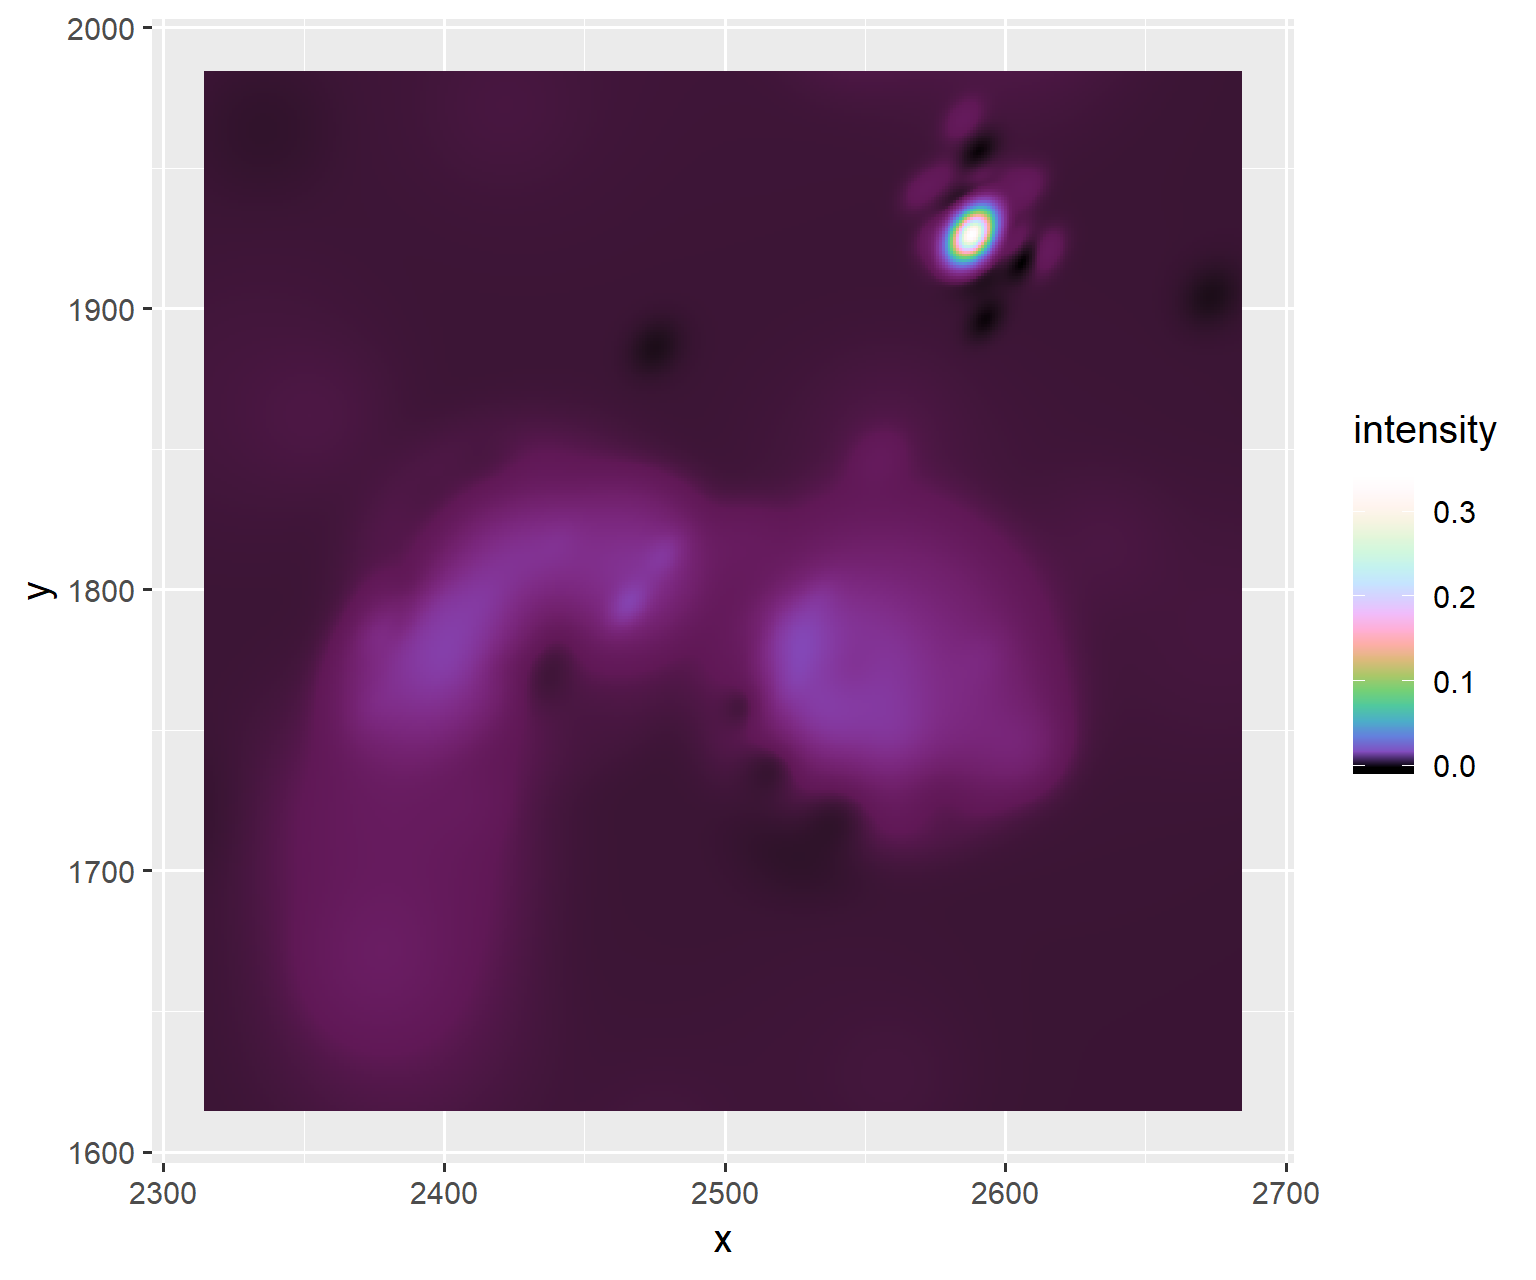
\includegraphics[width=1.00\linewidth]{./chapters/10.results/MSClean/Briggs-Calibration.png}
		\caption{Briggs CLEAN}
	\end{subfigure}
	\begin{subfigure}[b]{0.45\linewidth}
		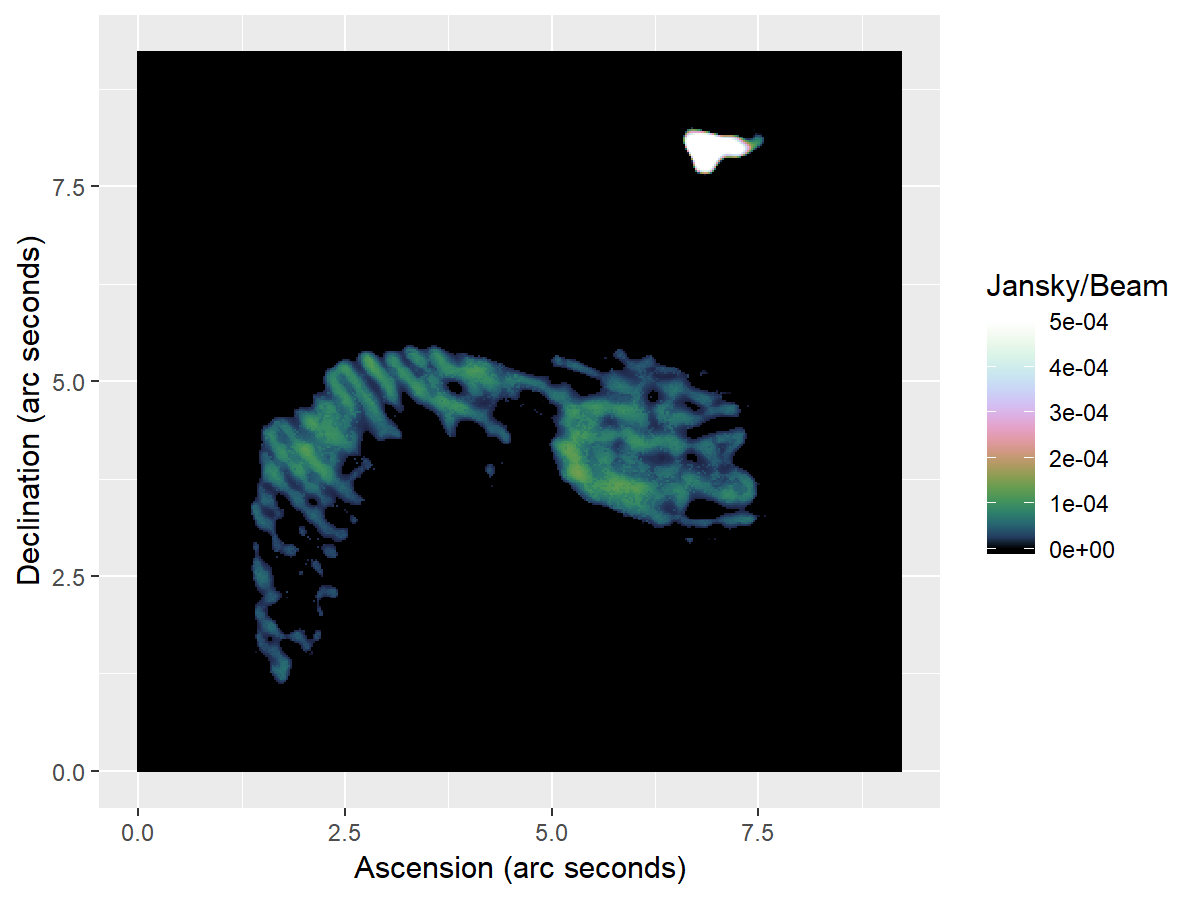
\includegraphics[width=1.00\linewidth]{./chapters/10.results/SerialCD/CD-Calibration.png}
		\caption{Coordinate Descent}
	\end{subfigure}
	\caption{Influence of calibration errors}
	\label{results:cleancomp::calib:figure}
\end{figure}

If we compare the reconstruction algorithm on areas with calibration errors, we clearly see that it negatively influences the reconstruction of serial coordinate descent. Figure \ref{results:cleancomp::calib:figure} shows a cutout of the right hand section of the reconstruction, where a faint extended emission is next to a point source with calibration errors. Multi-scale CLEAN is able to differentiate between the 'ripples' from the calibration error, and the extended emission. Coordinate descent with the elastic net regularization includes the ripples into the reconstructed image. 

The easiest way to exclude the calibration ripples from the reconstruction is to increase the regularization parameter $\lambda$, such as no pixel gets included which is not above the noise level + calibration error in the image. However, that would lead to other sources being "regularized away" in other regions of the image, which do not have a severe calibration error close by. 


\subsection{Serial coordinate descent speedup with MPI or GPU}\label{results:speedup}
In this section we test how much we can speed-up our serial coordinate descent algorithm by using distributed computing with MPI, or GPU acceleration.

We test the distributed serial coordinate descent on a shared memory system(Meaning all CPUs have access to the same main memory) with 32 CPUs. This is a best-case scenario for our implementation, because each node runs on the same physical machine: Our implementation needs a communication step between the nodes for each serial coordinate descent iteration. It needs a low-latency connection between each node to run as efficient as possible. Since each node runs on the same physical machine, it has a low latency times and therefore a low communication time. In this implementation, each node uses a single processor. We compare the speedup the algorithm achieves by adding more nodes/processors.

For the GPU we used personal computer level hardware, and tested on a nVidia Quadro M1200. We compare the speedup we achieve to the on-board CPU, which is an Intel Xeon E3-1505M with 8 logical processors at different image sizes. The speedup is shown in Figure \ref{results:speedup:figure}.

\begin{figure}[h]
	\centering
		\begin{subfigure}[b]{0.45\linewidth}
		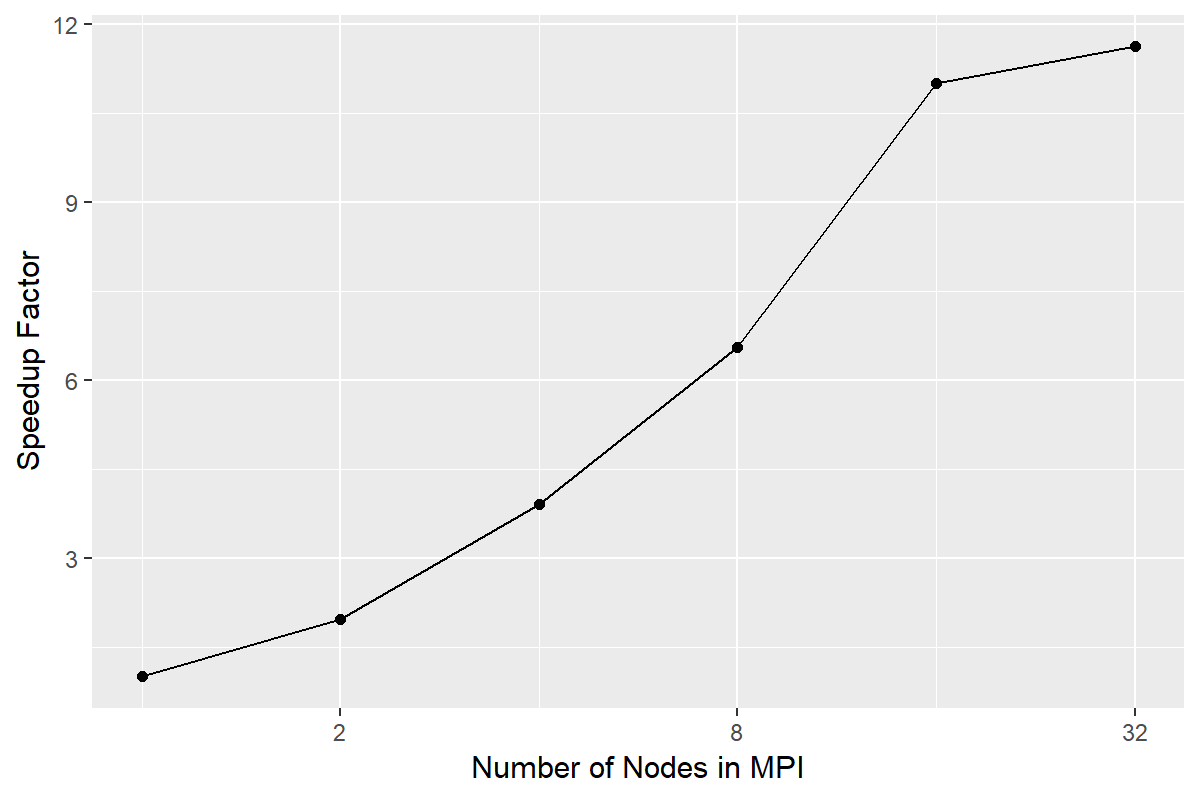
\includegraphics[width=1.00\linewidth]{./chapters/10.results/speedup/dist-speedup.png}
	\end{subfigure}
	\begin{subfigure}[b]{0.45\linewidth}
		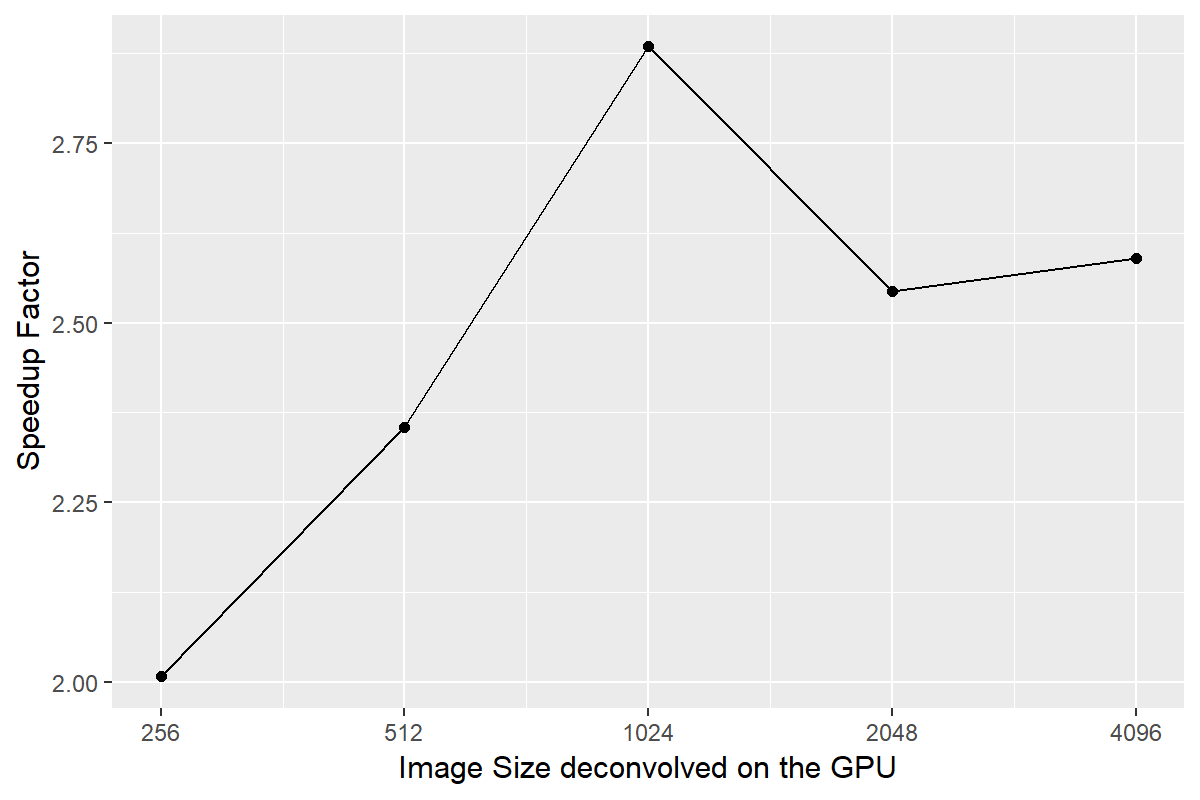
\includegraphics[width=1.00\linewidth]{./chapters/10.results/speedup/gpu.png}
	\end{subfigure}
	\caption{Speedup by using MPI or GPU acceleration}
	\label{results:speedup:figure}
\end{figure}

As we mentioned before, the speedup we achieve by using nodes/processors in MPI is the best-case scenario. As the best case scenario, we achieve a significant performance increase by using more nodes/processors. Up to 16 processors, the speedup we achieve is at least linear. Afterwards however the speedup diminishes. With 32 processors, we are only marginally faster than with 16. If the nodes would run two different physical machines, the speedup we achieve would depend mainly on the latency of the connection. 

The speedup we achieve by using GPU acceleration is fairly constant over the image size. The speedup factor varies around 2.5. Ideally, we would like to combine the distributed and the GPU implementation. However, this is not useful with the current implementation: The main bottleneck in the MPI implementation is the communication step in each iteration. 

We do not have a CLEAN implementation in our .Net Core pipeline. However, we mentioned the similarities between the serial coordinate descent and CLEAN in Section \ref{cd:similarities}. A single serial coordinate descent iteration is roughly equivalent to a standard CLEAN iteration. If we assume we need 14'000 CLEAN iterations to reconstruct an image, we can get a rough estimate by comparing the wall-clock time of 14'000 serial coordinate descent iterations. In this case, CLEAN is roughly 7 times faster than the current serial coordinate descent iteration.

Overall the serial coordinate descent algorithm with GPU acceleration is still several factors slower than CLEAN. The speedup we achieve with MPI is significant. But because serial coordinate descent and CLEAN have such a similar structure, we can expect a similar speedup with a CLEAN-MPI implementation. We need another method to speed up our deconvolution algorithm.


\subsection{Serial coordinate descent with an approximate $PSF$} \label{results:gradients}
In this section, we test our main hypothesis on the MeerKAT LMC data: The Major cycle allows us to use an approximation of the true $PSF$ in Minor cycle. We believe this can be exploited. We may be able to use a fraction of the true $PSF$ in the serial coordinate descent algorithm, potentially speeding up the deconvolution and simplifying distribution.

An example of the $PSF$ approximation is shown Figure \ref{results:gradients:clark}. Instead of the full $PSF$, we use a window around the center of the $PSF$. The sides of the window are a fraction of the full $PSF$.
\begin{figure}[h]
	\centering
	\begin{subfigure}[b]{0.245\linewidth}
		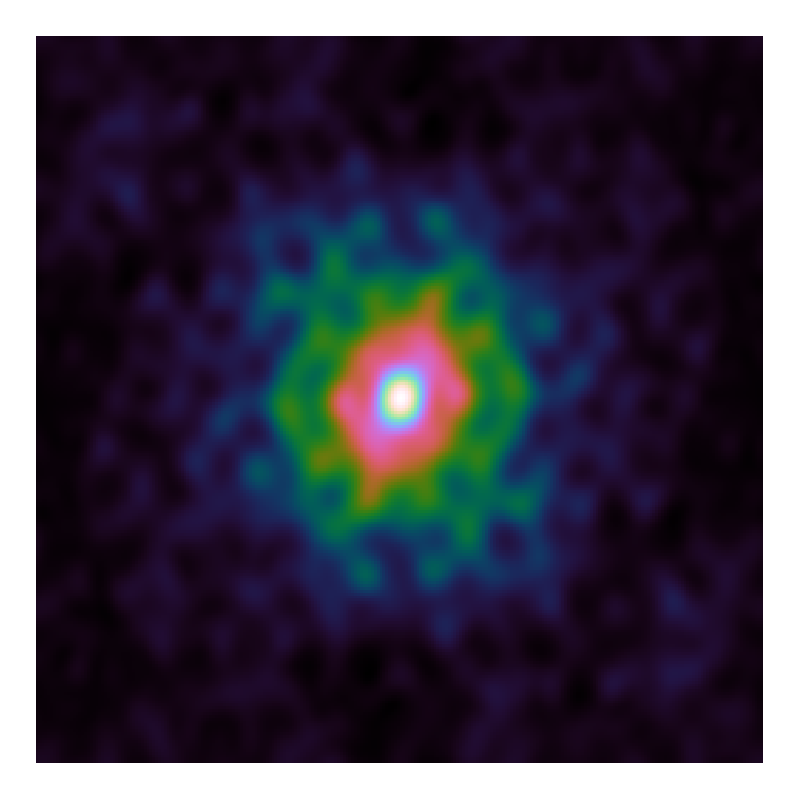
\includegraphics[width=\linewidth, clip, trim= 0.25in 0.25in 0.25in 0.25in]{./chapters/03.cd/simulated/psf.png}
		\caption{Full $PSF$}
	\end{subfigure}
	\begin{subfigure}[b]{0.245\linewidth}
		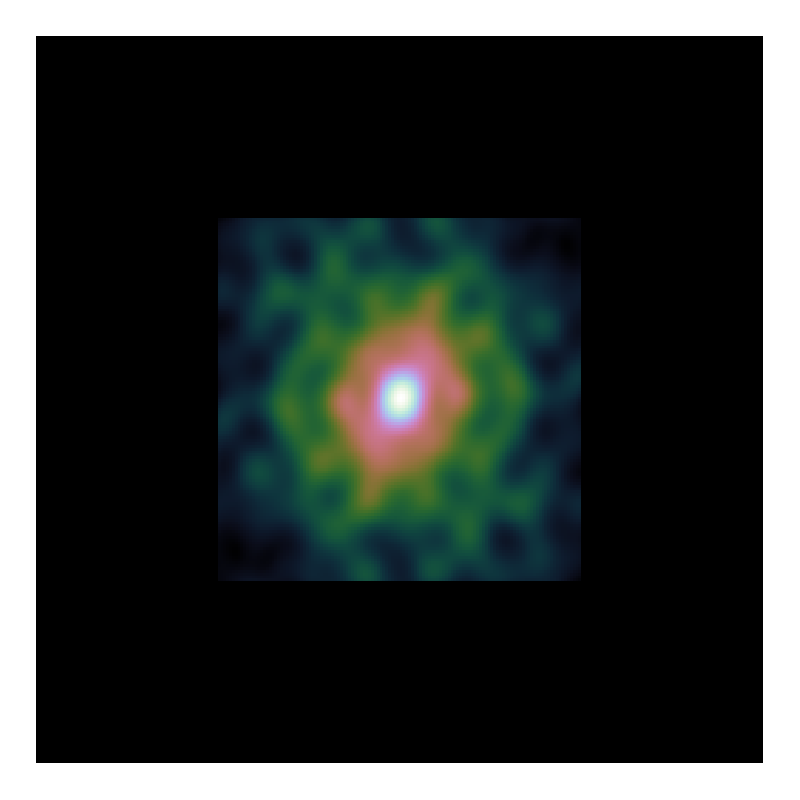
\includegraphics[width=\linewidth, clip, trim= 0.25in 0.25in 0.25in 0.25in]{./chapters/03.cd/simulated/psfCut.png}
		\caption{$\frac{1}{2}PSF$ approximation}
	\end{subfigure}
	\caption{Example of a $PSF$ approximation.}
	\label{results:gradients:clark}
\end{figure}

In this section, we test ever smaller window sizes and observe the convergence speed of our serial coordinate descent algorithm. We developed two methods to exploit an approximate $PSF$ in our serial coordinate descent algorithm: Method 1, approximate update and method 2, approximate deconvolution. At the start of each Major cycle, we calculate the objective value of the current solution, and track its development for each Major cycle. Finally, we combine the two approximation methods and compare how much we can speed up our serial coordinate descent method.


\subsubsection{Method 1: Approximate update}
As described in Section \ref{gradients:methods:update}, we normally use the product of $PSF \star PSF$ to update the gradient map in each iteration of serial coordinate descent. This method uses the approximate $PSF$ to update the gradient map: $Cut(PSF) \star Cut(PSF)$. With each iteration, the gradient map becomes less accurate. This approximation method is guaranteed to converge to the same result, if we have unlimited number of major cycles.
	
To test the convergence behaviour, we calculate the objective value of the current solution at the start of each Major cycle. We compare the objective value and the wall-clock time of the original serial coordinate descent and the serial coordinate descent using an approximate gradient update. This is a minimization problem, meaning the lowest objective is the most accurate reconstruction (according to the elastic net regularization).

\begin{figure}[h]
	\centering
	\begin{subfigure}[b]{0.58\linewidth}
		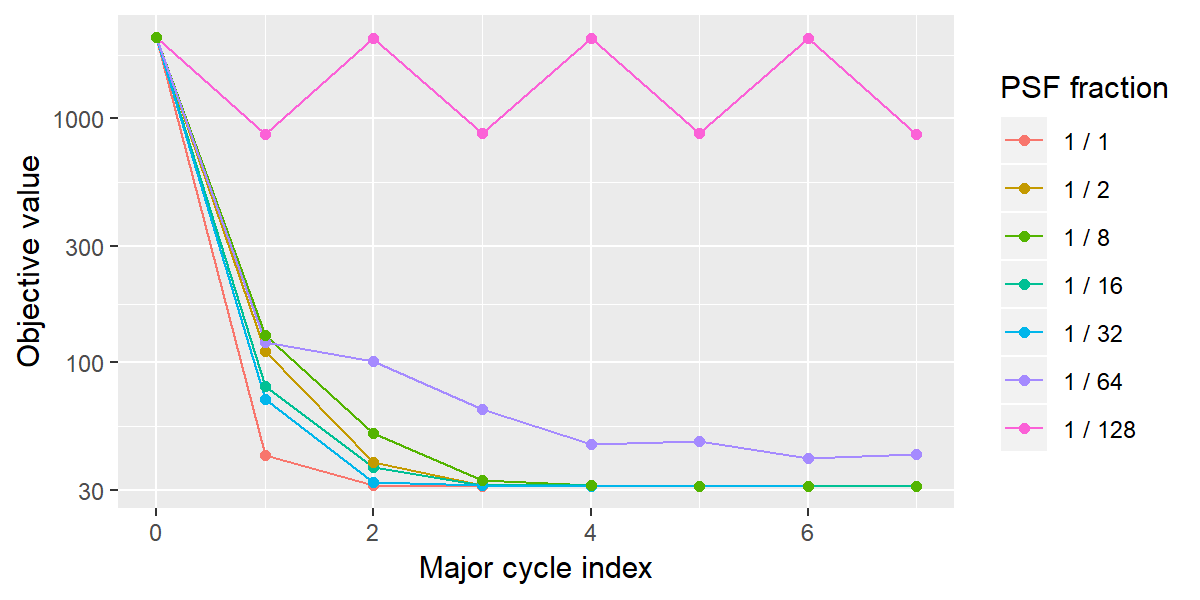
\includegraphics[width=\linewidth]{./chapters/10.results/gradient/ApproxUpdate/size.png}
	\end{subfigure}
	\begin{subfigure}[b]{0.195\linewidth}
		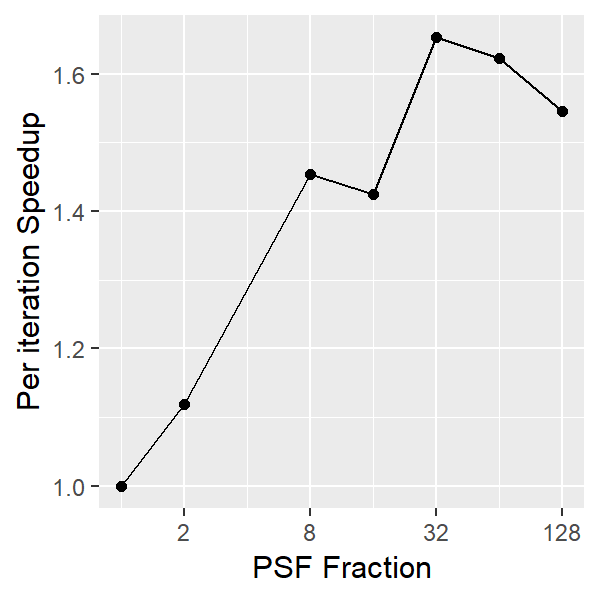
\includegraphics[width=\linewidth]{./chapters/10.results/gradient/ApproxUpdate/speedup_iter.png}
	\end{subfigure}
	\begin{subfigure}[b]{0.195\linewidth}
		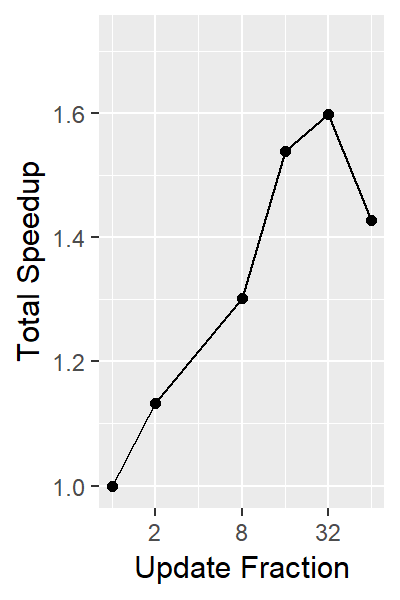
\includegraphics[width=\linewidth]{./chapters/10.results/gradient/ApproxUpdate/speedup_total.png}
	\end{subfigure}
	
	\caption{Convergence of the approx. update.}
	\label{results:gradients:update}
\end{figure}

Figure \ref{results:gradients:update} shows the convergence rate of the serial coordinate descent algorithm with the approximate update method. Each line represents a run with a specific $PSF$ window. The size of the window are a fraction of the full $PSF$. For example, the full $PSF$ in this test has $3072^2$ pixels. The approximation $\frac{1}{64}$ uses a window around the center of the $PSF$, which is is $48^2$ pixels in size. The $\frac{1}{64}$  approximation is uses the smallest window around the $PSF$ for which the serial coordinate descent algorithm still converges. If we use less aggressive approximations, we see the serial coordinate descent algorithm reach a similar objective value within three Major cycles. 

We compare two different wall-clock times: The average time necessary for a single serial coordinate descent iteration, and the total time spent in the algorithm. We see from the two speedup curves in Figure \ref{results:gradients:update} that the speedup per iteration increases less than linear with the $PSF$ fraction used in the approximation. Although each iteration becomes cheaper with a smaller $PSF$ window, we may need more iterations to converge to the same result. This is indeed the case for a $PSF$ window smaller than $\frac{1}{32}$. We see a significant drop total speedup. Overall with gradient update approximations give us a speedup factor of 1.6, if we use $\frac{1}{32}$ of the full $PSF$.


\subsubsection{Method 2: Approximate deconvolution}
As described in Section \ref{gradients:methods:deconv}, this approximation method uses the same approximation to update the gradient map($Cut(PSF) \star Cut(PSF)$). This approximation method also uses the approximate $PSF$ to initialize the gradient map: $gradients = residuals \star Cut(PSF)$. As such, this approximation method deconvolves the image not with the full $PSF$, but with the center window. This method is not guaranteed to converge to the same result. Nevertheless, we run our serial coordinate descent algorithm on different $PSF$ fractions and compare the true objective value at the start of each Major cycle. The results are shown in Figure \ref{results:gradients:aproxDeconv}.

\begin{figure}[h]
	\centering
	\begin{subfigure}[b]{0.58\linewidth}
		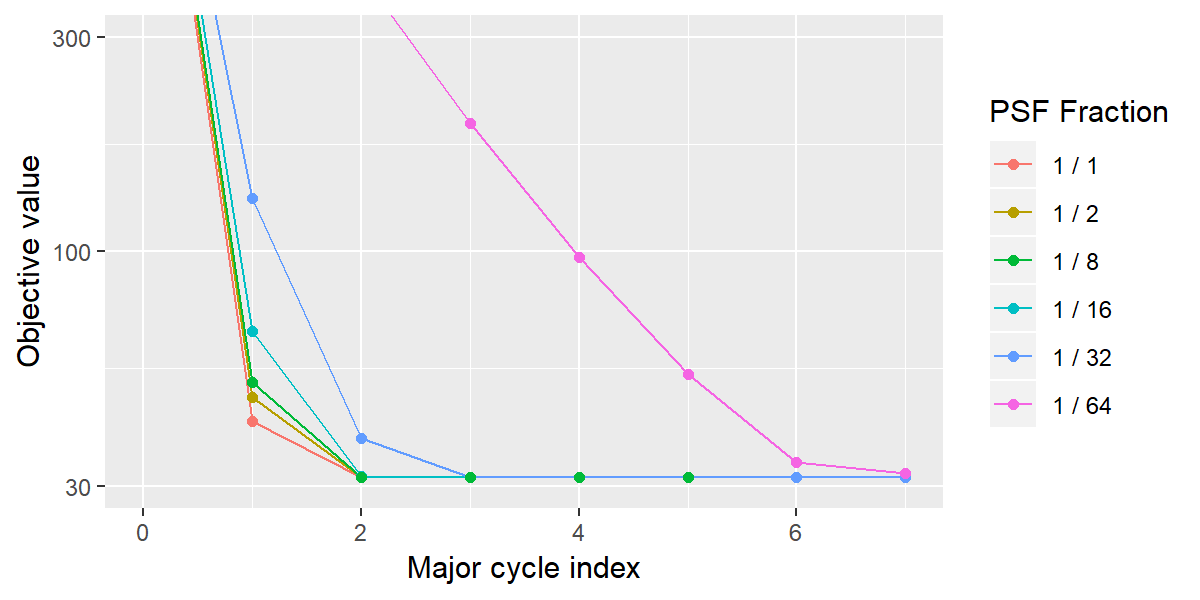
\includegraphics[width=\linewidth]{./chapters/10.results/gradient/ApproxDeconv/size.png}
	\end{subfigure}
	\begin{subfigure}[b]{0.195\linewidth}
		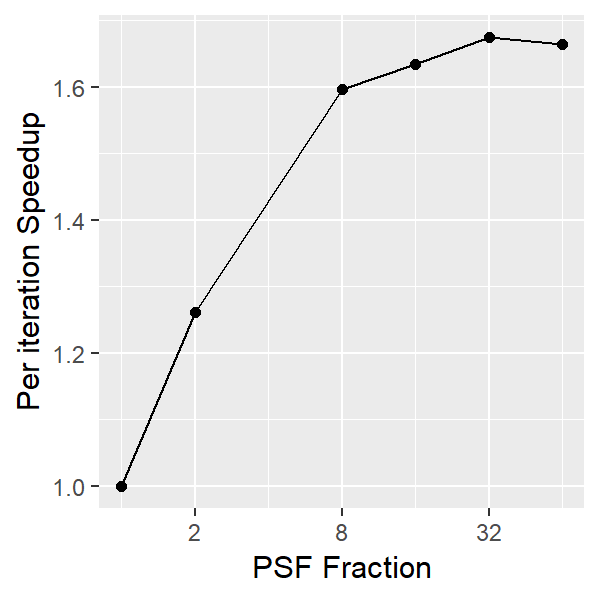
\includegraphics[width=\linewidth]{./chapters/10.results/gradient/ApproxDeconv/speedup_iter.png}
	\end{subfigure}
	\begin{subfigure}[b]{0.195\linewidth}
		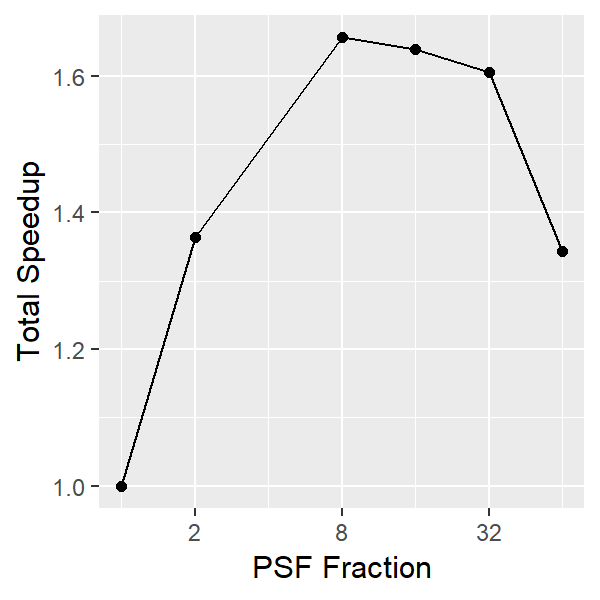
\includegraphics[width=\linewidth]{./chapters/10.results/gradient/ApproxDeconv/speedup_total.png}
	\end{subfigure}
	
	\caption{Effect of the L1 and L2 Norm separately.}
	\label{results:gradients:aproxDeconv}
\end{figure}

Again, the smallest window for which the serial coordinate descent algorithm converges is $\frac{1}{64}$. Similar to method 1, the serial coordinate descent algorithm reaches a similar objective value within 3 Major cycles, for all $PSF$ windows except $\frac{1}{64}$. The total speedup however is notably different: It reaches a larger total speedup. The total speedup curve generally matches better with the 'per iteration speedup' curve. This suggests that the approximate deconvolution method does not require significantly more iterations to converge, even when we use a $PSF$ window of $\frac{1}{16}$. 

The approximate deconvolution method is not guaranteed to lead to the same result. Nevertheless, the true objective value of the results are practically identical in Figure \ref{results:gradients:aproxDeconv}. However, as we mentioned before, this approximation method systematically under-estimates the true pixel values. The pixel magnitude is important in the self-calibration regime \cite{offringa2017optimized}. Self-calibration uses intermediate results of the image reconstruction to improve the calibration. A systematic under-estimation of the pixel values leads to a bias in self-calibration.


\subsubsection{Combination of Method 1 and 2}\label{results:gradients:comparison}
The approximation method 2, approximate deconvolution, leads to a systematic under-estimation of the true pixel values. This is undesirable for a reconstruction algorithm. The obvious question is, how does the serial coordinate descent algorithm perform when we combine the two approximation methods: We start with method 2. When the algorithm converged, we switch to method 1 and correct the systematic error introduced by method 2. We compare the speedup we achieve by combining the two approximation methods in Table \ref{results:gradients:comparison:speedup}.


\begin{table}[h]
	\centering
	\begin{tabular}{ c | c ||c|c } 
		\hline
		Method & $PSF$ Fraction & Iteration Speedup & Total Speedup \\ \hline \hline
		Original & $\frac{1}{16}$ & 1.00 & 1.00 \\ 
		(Method 1) Approx. gradient update & $\frac{1}{16}$ & 1.66 & 1.55 \\ 
		(Method 2) Approx. deconvolution & $\frac{1}{16}$ & 1.67 & 1.68 \\ \hline
		Combined & $\frac{1}{16}$ & 1.69 & 1.68 \\ 
		\hline
	\end{tabular}

	\caption{Results when combining the two approximation methods}
	\label{results:gradients:comparison:speedup}
	
\end{table}

Combining the two approximation methods leads to a total speedup with a $PSF$ window of $\frac{1}{16}$. The combined approximation method achieves a larger speedup than method 1 or method 2 on the same $PSF$ window size. We suspect the error each approximation method introduces is uncorrelated. Meaning the error we introduce with approximation method 2 can be efficiently corrected with approximation method 1, which leads to a higher total speedup.


\begin{figure}[h]
	\centering
	\begin{subfigure}[b]{0.3\linewidth}
		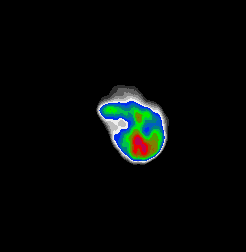
\includegraphics[width=1.00\linewidth]{./chapters/10.results/cleancomp/n132_cd.png}
		\\
		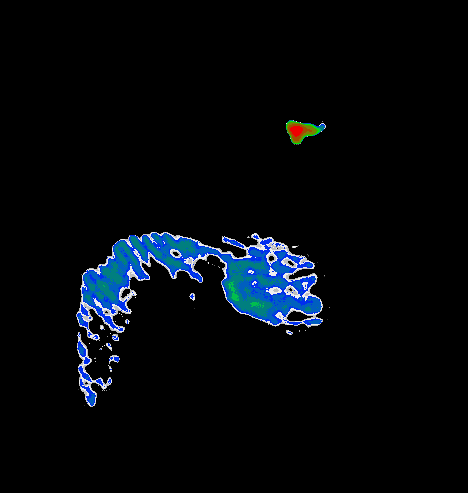
\includegraphics[width=1.00\linewidth]{./chapters/10.results/cleancomp/cd_calibration.png}
		\caption{Original CD}
	\end{subfigure}
	\begin{subfigure}[b]{0.3\linewidth}
		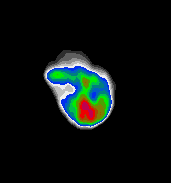
\includegraphics[width=1.00\linewidth]{./chapters/10.results/gradient/combined/combined_n132d.png}
		\\
		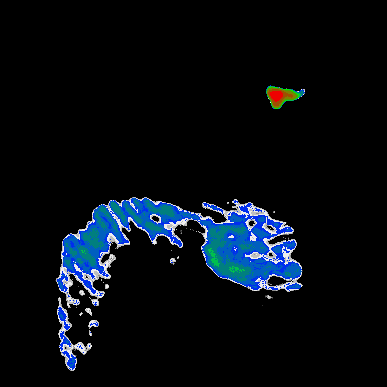
\includegraphics[width=1.00\linewidth]{./chapters/10.results/gradient/combined/combined_calibration.png}
		\caption{Combined approximation}
	\end{subfigure}

	\caption{Image comparison to approximation}
	\label{results:gradients:comparison:image}
\end{figure}

Figure \ref{results:gradients:comparison:image} compares the original result with the result of the combined approximation. Virtually identical. Same problem with calibration. Only visual difference in the extended emission with calibration errors. 




